\documentclass[10pt]{article}
\usepackage[utf8]{inputenc}
\usepackage[export]{adjustbox}
\usepackage{longtable}
\usepackage{geometry}
\usepackage{amsfonts}
\usepackage{hyperref}
\usepackage{enumitem}
\usepackage{graphicx}
\usepackage{tabularx}
\usepackage{amsmath}
\usepackage{xcolor}


\newcommand{\unit}[1]{\mathbf{\hat{#1}}}
\newcommand{\orientation}[1]{\left[ \mathbf{R}_{#1} \mid \mathbf{t}_{#1} \right]}
\newcommand{\figref}[1]{Figure (\ref{fig:#1})}


\title{
    \textbf{CSE344: Computer Vision} \\ \vspace*{-5pt}
    \textbf{\large{Assignment-2}}
}

\author{\href{mailto:divyajeet21529@iiitd.ac.in}{Divyajeet Singh (2021529)}}
\date{\today}

\geometry{a4paper, left=20mm, right=20mm, top=20mm, bottom=20mm}


\begin{document}
    \maketitle

    \section*{\textbf{Question 1.}}
    \begin{enumerate}
        \item The given transformation is a composition of the following three transformations
        (in order):
        \begin{enumerate}[label=(\alph*)]
            \item Rotation by $\frac{\pi}{2}$ about the $Y$-axis
            \item Rotation by $\frac{-\pi}{2}$ about the $X$-axis
            \item Translation by $t = \begin{bmatrix} -1 & 3 & 2 \end{bmatrix}^{\top}$
        \end{enumerate}
        The coordinate transformation matrices (using 3-dimensional homogeneous coordinates),
        for the three transformations are
        \begin{align*}
            R_{y}\left(\frac{\pi}{2}\right) &= \begin{bmatrix}
                \cos{\left(\frac{\pi}{2}\right)} & 0 & \sin{\left(\frac{\pi}{2}\right)} & 0 \\
                0 & 1 & 0 & 0 \\
                -\sin{\left(\frac{\pi}{2}\right)} & 0 & \cos{\left(\frac{\pi}{2}\right)} & 0 \\
                0 & 0 & 0 & 1
            \end{bmatrix} = \begin{bmatrix}
                0 & 0 & 1 & 0 \\
                0 & 1 & 0 & 0 \\
                -1 & 0 & 0 & 0 \\
                0 & 0 & 0 & 1
            \end{bmatrix} \\
            R_{x}\left(\frac{-\pi}{2}\right) &= \begin{bmatrix}
                1 & 0 & 0 & 0 \\
                0 & \cos{\left(\frac{-\pi}{2}\right)} & -\sin{\left(\frac{-\pi}{2}\right)} & 0 \\
                0 & \sin{\left(\frac{-\pi}{2}\right)} & \cos{\left(\frac{-\pi}{2}\right)} & 0 \\
                0 & 0 & 0 & 1
            \end{bmatrix} = \begin{bmatrix}
                1 & 0 & 0 & 0 \\
                0 & 0 & 1 & 0 \\
                0 & -1 & 0 & 0 \\
                0 & 0 & 0 & 1
            \end{bmatrix} \\
            T(t) &= \begin{bmatrix}
                1 & 0 & 0 & -1 \\
                0 & 1 & 0 & 3 \\
                0 & 0 & 1 & 2 \\
                0 & 0 & 0 & 1
            \end{bmatrix}
        \end{align*}
        The coordinate transformation matrix for the full transformation is then given by
        \begin{align*}
            T &= T(t) \circ R_{x}\left(\frac{-\pi}{2}\right) \circ R_{y}\left(\frac{\pi}{2}\right) \\
            &= T(t) \begin{bmatrix}
                1 & 0 & 0 & 0 \\
                0 & 0 & 1 & 0 \\
                0 & -1 & 0 & 0 \\
                0 & 0 & 0 & 1
            \end{bmatrix} \begin{bmatrix}
                0 & 0 & 1 & 0 \\
                0 & 1 & 0 & 0 \\
                -1 & 0 & 0 & 0 \\
                0 & 0 & 0 & 1
            \end{bmatrix} \\
            &= \begin{bmatrix}
                1 & 0 & 0 & -1 \\
                0 & 1 & 0 & 3 \\
                0 & 0 & 1 & 2 \\
                0 & 0 & 0 & 1
            \end{bmatrix} \begin{bmatrix}
                0 & 0 & 1 & 0 \\
                -1 & 0 & 0 & 0 \\
                0 & -1 & 0 & 0 \\
                0 & 0 & 0 & 1
            \end{bmatrix} = \begin{bmatrix}
                0 & 0 & 1 & -1 \\
                -1 & 0 & 0 & 3 \\
                0 & -1 & 0 & 2 \\
                0 & 0 & 0 & 1
            \end{bmatrix}
        \end{align*}
        since rotations and translations are linear transformations in homogeneous
        coordinate systems, and hence composition of transformations is equivalent
        to multiplication of the transformation matrices.

        \item Now, we find the new coordinates of a given vector,
        $v = \begin{bmatrix} 2 & 5 & 1 \end{bmatrix}^{\top}$, after the transformation.
        The new coordinates, say $v'$, are given by simply applying the transformation
        matrix to $v$ in homogeneous coordinates, which gives
        \begin{equation*}
            v' = T v = \begin{bmatrix}
                0 & 0 & 1 & -1 \\
                -1 & 0 & 0 & 3 \\
                0 & -1 & 0 & 2 \\
                0 & 0 & 0 & 1
            \end{bmatrix} \begin{bmatrix} 2 \\ 5 \\ 1 \\ 1 \end{bmatrix} = \begin{bmatrix}
                0 \\
                1 \\
                -3 \\
                1
            \end{bmatrix}
        \end{equation*}
        So, the new coordinates of the given vector are
        $v' = \begin{bmatrix} 0 & 1 & -3 \end{bmatrix}^{\top}$. We also find the point
        that the origin of the initial frame of reference gets mapped to. For this, we
        simply apply the transformation matrix $T$ to the origin $\mathbf{0}$ in homogeneous
        coordinates, which gives
        \begin{equation*}
            T \mathbf{0} = \begin{bmatrix}
                0 & 0 & 1 & -1 \\
                -1 & 0 & 0 & 3 \\
                0 & -1 & 0 & 2 \\
                0 & 0 & 0 & 1
            \end{bmatrix} \begin{bmatrix} 0 \\ 0 \\ 0 \\ 1 \end{bmatrix} = \begin{bmatrix}
                -1 \\
                3 \\
                2 \\
                1
            \end{bmatrix}
        \end{equation*}
        So, the origin gets mapped to the point $\begin{bmatrix} -1 & 3 & 2 \end{bmatrix}^{\top}$.
        In fact, the origin is invariant to pure rotations about the coordinate axes, so intuitively,
        the origin maps to the translation vector $t$.

        \item We now have the combined rotation matrix, $\mathbf{R}$ (written without homogeneous
        coordinates), as
        \begin{equation*}
            \mathbf{R} = \begin{bmatrix}
                0 & 0 & 1 \\
                -1 & 0 & 0 \\
                0 & -1 & 0
            \end{bmatrix}
        \end{equation*}
        Using Rodrigues formula, we can obtain the direction of the axis of this combined
        rotation in the original frame of reference and the angle of rotation about this axis.
        According to the Rodrigues formula, the angle of rotation is given by
        \begin{equation*}
            \theta = \cos^{-1}{\left(\frac{\textsc{Trace}(\mathbf{R}) - 1}{2}\right)}
            = \cos^{-1}{\left(\frac{-1}{2}\right)} = \frac{2\pi}{3}
        \end{equation*}
        The axis of rotation, $\unit{n}$, is given by
        \begin{equation*}
            \unit{n} = \frac{1}{2\sin{\theta}} \begin{bmatrix}
                \mathbf{R}_{32} - \mathbf{R}_{23} \\
                \mathbf{R}_{13} - \mathbf{R}_{31} \\
                \mathbf{R}_{21} - \mathbf{R}_{12}
            \end{bmatrix}
            = \frac{1}{2\sin{\frac{2\pi}{3}}} \begin{bmatrix}
                -1 - 0 \\
                1 - 0 \\
                -1 - 0
            \end{bmatrix} = \frac{1}{\sqrt{3}} \begin{bmatrix}
                -1 \\
                1 \\
                -1
            \end{bmatrix}
        \end{equation*}
        Therefore, the combined rotation is a rotation of $\frac{2\pi}{3}$ about the axis
        $\frac{1}{\sqrt{3}} \begin{bmatrix} -1 & 1 & -1 \end{bmatrix}^{\top}$,
        i.e.
        \begin{equation*}
            \mathbf{R} \equiv R\left(\frac{1}{\sqrt{3}} \begin{bmatrix}
                -1  \\
                1 \\
                -1
            \end{bmatrix}, \frac{2\pi}{3}\right)
        \end{equation*}

        \item We now use the above axis $\unit{n}$ and angle $\theta$ to calculate the
        the rotation matrix (say) $\mathbf{R'}$ for the rotation, and show that it is the
        same as matrix $\mathbf{R}$ that we obtained through sequentially applying the two
        given rotations. Using the Rodrigues formula, the rotation matrix $\mathbf{R'}$ is
        given by
        \begin{equation*}
            \mathbf{R'} = \mathbf{I} + \sin{\theta} \mathbf{N} + (1 - \cos{\theta}) \mathbf{N}^2
            \quad \text{where} \quad \mathbf{N} = \begin{bmatrix}
                0 & -n_{3} & n_{2} \\
                n_{3} & 0 & -n_{1} \\
                -n_{2} & n_{1} & 0
            \end{bmatrix} \quad (n_{i} \text{ represent the components of } \unit{n})
        \end{equation*}
        We first find $\mathbf{N}$ and then use it to find $\mathbf{R'}$. We have
        \begin{equation*}
            \mathbf{N} =  \frac{1}{\sqrt{3}} \begin{bmatrix}
                0 & 1 & 1 \\
                -1 & 0 & 1 \\
                -1 & -1 & 0
            \end{bmatrix} \implies \mathbf{N}^{2} = \frac{1}{3} \begin{bmatrix}
                -2 & -1 & 1 \\
                -1 & -2 & -1 \\
                1 & -1 & -2
            \end{bmatrix} \\
        \end{equation*}
        Using these, we find
        \begin{align*}
            \mathbf{R'} &= \begin{bmatrix}
                1 & 0 & 0 \\
                0 & 1 & 0 \\
                0 & 0 & 1
            \end{bmatrix} + \frac{1}{\sqrt{3}} \sin{\frac{2\pi}{3}} \begin{bmatrix}
                0 & 1 & 1 \\
                -1 & 0 & 1 \\
                -1 & -1 & 0
            \end{bmatrix} + \frac{1}{3} \left(1 - \cos{\frac{2\pi}{3}} \right) \begin{bmatrix}
                -2 & -1 & 1 \\
                -1 & -2 & -1 \\
                1 & -1 & -2
            \end{bmatrix} \\
            &= \begin{bmatrix}
                1 & 0 & 0 \\
                0 & 1 & 0 \\
                0 & 0 & 1
            \end{bmatrix} + \frac{1}{2} \begin{bmatrix}
                0 & 1 & 1 \\
                -1 & 0 & 1 \\
                -1 & -1 & 0
            \end{bmatrix} + \frac{1}{2} \begin{bmatrix}
                -2 & -1 & 1 \\
                -1 & -2 & -1 \\
                1 & -1 & -2
            \end{bmatrix} \\
            &= \begin{bmatrix}
                0 & 0 & 1 \\
                -1 & 0 & 0 \\
                0 & -1 & 0
            \end{bmatrix} = \mathbf{R}
        \end{align*}
        Hence, we have shown that the rotation matrix $\mathbf{R'}$ obtained using the axis
        $\unit{n}$ and angle $\theta$ is the same as the matrix $\mathbf{R}$ that we obtained
        through sequentially applying the two given rotations. This also proves the correctness
        of the axis and angle obtained using the Rodrigues formula.
    \end{enumerate}

    \section*{\textbf{Question 2.}}
    By Rodrigues formula, we know that the rotated vector for the given rotation is
    given by
    \begin{align*}
        \mathbf{R} \mathbf{x} &= \mathbf{x} + (\unit{u} \times \mathbf{x}) \sin{\theta}
        + (1 - \cos{\theta}) \unit{u} \times (\unit{u} \times \mathbf{x}) \\
        &= \mathbf{x} + (\unit{u} \times \mathbf{x}) \sin{\theta}
        + (1 - \cos{\theta}) \left[ (\unit{u}^{\top} \mathbf{x}) \unit{u} - (\unit{u}^{\top}
        \unit{u}) \mathbf{x} \right] \\
        &= \mathbf{x} + (\unit{u} \times \mathbf{x}) \sin{\theta}
        + (1 - \cos{\theta}) (\unit{u}^{\top} \mathbf{x}) \unit{u} - (1 - \cos{\theta})
        \mathbf{x} \\
        &= \mathbf{x} - \mathbf{x} + \mathbf{x} \cos{\theta} + (\unit{u} \times \mathbf{x})
        \sin{\theta} + (1 - \cos{\theta}) (\unit{u}^{\top} \mathbf{x}) \unit{u} \\
        &= \mathbf{x} \cos{\theta} + (\unit{u} \times \mathbf{x}) \sin{\theta}
        + (\unit{u}^{\top} \mathbf{x}) (1 - \cos{\theta}) \unit{u} \tag*{$\square$}
    \end{align*}
    which proves the result, using the vector triple product identity that states
    for any vectors $\mathbf{a}$, $\mathbf{b}$, and $\mathbf{c}$,
    \begin{equation*}
        \mathbf{a} \times (\mathbf{b} \times \mathbf{c}) = (\mathbf{a}^{\top} \mathbf{c})
        \mathbf{b} - (\mathbf{a}^{\top} \mathbf{b}) \mathbf{c}
    \end{equation*}
    and that $\unit{u}^{\top} \unit{u} = 1$ since $\unit{u}$ is a unit vector.

    \section*{\textbf{Question 3.}}
    We are given image formation equations of two cameras, $\mathbf{C}_{1}$ and
    $\mathbf{C}_{2}$, for the same 3D point $\mathbf{X}$ in the world in homogeneous
    coordinates, as follows
    \begin{align*}
        \mathbf{x}_{1} &= \mathbf{K}_{1} \orientation{1} \mathbf{X} \\
        \mathbf{x}_{2} &= \mathbf{K}_{2} \orientation{2} \mathbf{X}
    \end{align*}
    where we assume that the extrinsic matrices
    $\left[ \mathbf{R}_{i} \mid \mathbf{t}_{i} \right]_{3 \times 4}$, include the perspective projection
    matrix $\begin{bmatrix} \mathbf{I} & \mathbf{0} \end{bmatrix}$. We need to show that the image
    points are related by
    \begin{equation*}
        \mathbf{x}_{1} = \mathbf{H} \mathbf{x}_{2}
    \end{equation*}
    for some invertible $\mathbf{H}_{3 \times 3}$ and find it in terms of $\mathbf{K}_{1}$,
    $\mathbf{K}_{2}$, and $\mathbf{R}$. \\
    Given that the orientation of $\mathbf{C}_{2}$ is obtained by applying a 3D rotation
    $\mathbf{R}$ on $\mathbf{C}_{1}$, which means
    \begin{equation*}
        \orientation{2} = \mathbf{R} \orientation{1}
   \end{equation*}
    Then, we have
    \begin{align*}
            \mathbf{x}_{1} &= \mathbf{H} \mathbf{x}_{2} \\
            \mathbf{x}_{1} &= \mathbf{H} \mathbf{K}_{2} \orientation{2} \mathbf{X} \\
            \mathbf{K}_{1} \orientation{1} \mathbf{X} &= \mathbf{H} \mathbf{K}_{2} \mathbf{R}
            \orientation{1} \mathbf{X} \\
            \implies \mathbf{K}_{1} \orientation{1} &= \mathbf{H} \mathbf{K}_{2} \mathbf{R} \orientation{1}
            \quad \text{since } \mathbf{X} \text{ is arbitrary}
    \end{align*}
    At this point, it is important to consider the shapes of the matrices involved. We have
    \begin{equation*}
        \underbrace{\mathbf{K}_{1}}_{3 \times 3} \underbrace{\orientation{1}}_{3 \times 4} =
        \underbrace{\mathbf{H}}_{3 \times 3} \underbrace{\mathbf{K}_{2}}_{3 \times 3}
        \underbrace{\mathbf{R}}_{3 \times 3} \underbrace{\orientation{1}}_{3 \times 4}
    \end{equation*}
    Note that $\orientation{1}$ is not invertible. However, we do not need to invert it. Since the
    operands to the right remain the same, it is sufficient to find $\mathbf{H}$ such that the
    \begin{align*}
        \mathbf{K}_{1} &= \mathbf{H} \mathbf{K}_{2} \mathbf{R} \\
        \implies \mathbf{K}_{1} \mathbf{R}^{\top} &= \mathbf{H} \mathbf{K}_{2} \\
        \implies \mathbf{K}_{1} \mathbf{R}^{\top} \mathbf{K}_{2}^{-1} &= \mathbf{H}
    \end{align*}
    Therefore, the matrix $\mathbf{H} = \mathbf{K}_{1} \mathbf{R}^{\top} \mathbf{K}_{2}^{-1}$ gives the
    required relation between the image points. Finally, we show two properties of $\mathbf{H}$
    \begin{enumerate}
        \item $\mathbf{H}$ is of size $3 \times 3$. This is easy to see as
        \begin{equation*}
            \underbrace{\mathbf{H}}_{3 \times 3} = \underbrace{\mathbf{K}_{1}}_{3 \times 3}
            \underbrace{\mathbf{R}^{\top}}_{3 \times 3} \underbrace{\mathbf{K}_{2}^{-1}}_{3 \times 3}
        \end{equation*}

        \item $\mathbf{H}$ is invertible. This is also easy to see as
        \begin{equation*}
            \mathbf{H}^{-1} = \left( \mathbf{K}_{1} \mathbf{R}^{\top} \mathbf{K}_{2}^{-1} \right)^{-1}
            = \mathbf{K}_{2} \mathbf{R} \mathbf{K}_{1}^{-1}
        \end{equation*}
        where we crucially use the fact that $\mathbf{R}$ is an orthogonal matrix, and $\mathbf{K}_{1}$
        and $\mathbf{K}_{2}$ are invertible since they are upper triangular matrices with non-zero
        entries (number of pixels) on their principal diagonals.
    \end{enumerate}
    We can verify the correctness of the result by substituting the obtained $\mathbf{H}$ into the
    required relation. We have
    \begin{align*}
        \mathbf{x}_{1} &= \mathbf{H} \mathbf{x}_{2} \\
        &= \mathbf{K}_{1} \mathbf{R}^{\top} \mathbf{K}_{2}^{-1} \mathbf{x}_{2} \\
        &= \mathbf{K}_{1} \mathbf{R}^{\top} \mathbf{K}_{2}^{-1} \mathbf{K}_{2} \orientation{2} \mathbf{X} \\
        &= \mathbf{K}_{1} \mathbf{R}^{\top} \orientation{2} \mathbf{X} \\
        &= \mathbf{K}_{1} \orientation{1} \mathbf{X} \\
        &= \mathbf{x}_{1}
    \end{align*}
    since $\orientation{2} = \mathbf{R} \orientation{1} \implies \mathbf{R}^{\top} \orientation{2} = \orientation{1}$.

    \section*{\textbf{Question 4. (Camera Calibration)}}
    We are required to perform Camera Calibration with a set of 25 images of
    a chessboard pattern. A chessboard pattern of size $5 \times 7$ (given in
    [1]) was used for the calibration. The final set of images used for the
    camera calibration is given in \figref{final-image-set}. The images
    are numbered 1 to 25 from top-left to bottom-right. The resolution of the
    images is $4032 \times 3024$. \\
    The images were taken by placing the chessboard pattern on a flat surface
    and capturing the images from different angles and distances, capturing all
    degrees of freedom, esuring that the corners are clearly visible in each image.
    The code for this question is given in \texttt{camera-calibration.ipynb}.
    \begin{figure}[htbp]
        \begin{center}
            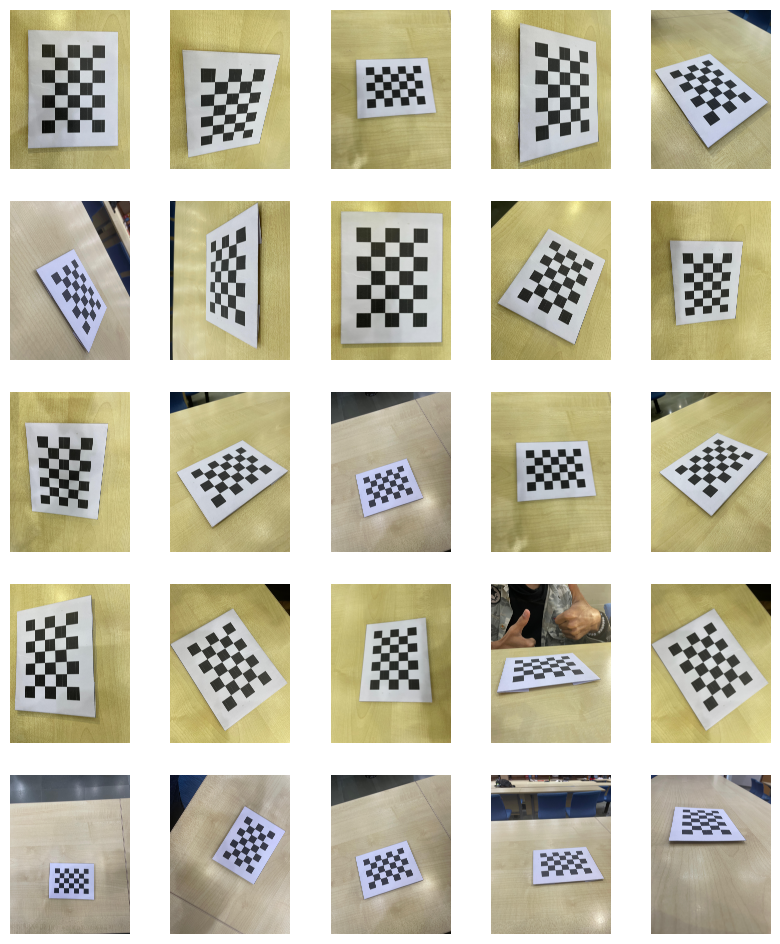
\includegraphics[width=0.875\textwidth]{Assets/Question-4/final-image-set.png}
            \caption{Chessboard pattern used for camera calibration}
            \label{fig:final-image-set}
        \end{center}
    \end{figure}
    \begin{enumerate}
        \item We estimate the intrinsic camera parameters using the images. The following
        intrinsic matrix was obtained.
        \begin{equation*}
            \mathbf{K} = \begin{bmatrix}
                f_{x} & s & c_{x} \\
                0 & f_{y} & c_{y} \\
                0 & 0 & 1
            \end{bmatrix} = \begin{bmatrix}
                3127.88 & 0.0 & 1508.31 \\
                0.0 & 3122.10 & 2013.85 \\
                0 & 0 & 1
            \end{bmatrix}
        \end{equation*}
        inidicating that (rounded off to the nearest integer) the focal length in the
        $x$ and $y$ directions is $f_{x} \approx 3128$ and $f_{y} \approx 3122$  respectively.
        The principal point is $(c_{x}, c_{y}) \approx (1508, 2014)$. The skew parameter is
        $s = 0$.

        \item We estimate the extrinsic camera parameters for each of the 25 images. A few of
        the results are given in Table \ref{tab:extrinsic-parameters}. The figures are rounded
        off to one decimal place for brevity. The precise parameters for each image can be found
        in the notebook.
        \begin{longtable}{c|c|c}
            \textsc{Image} & \textsc{Rotation Matrix} & \textsc{Translation Vector} \\
            \hline & & \\
            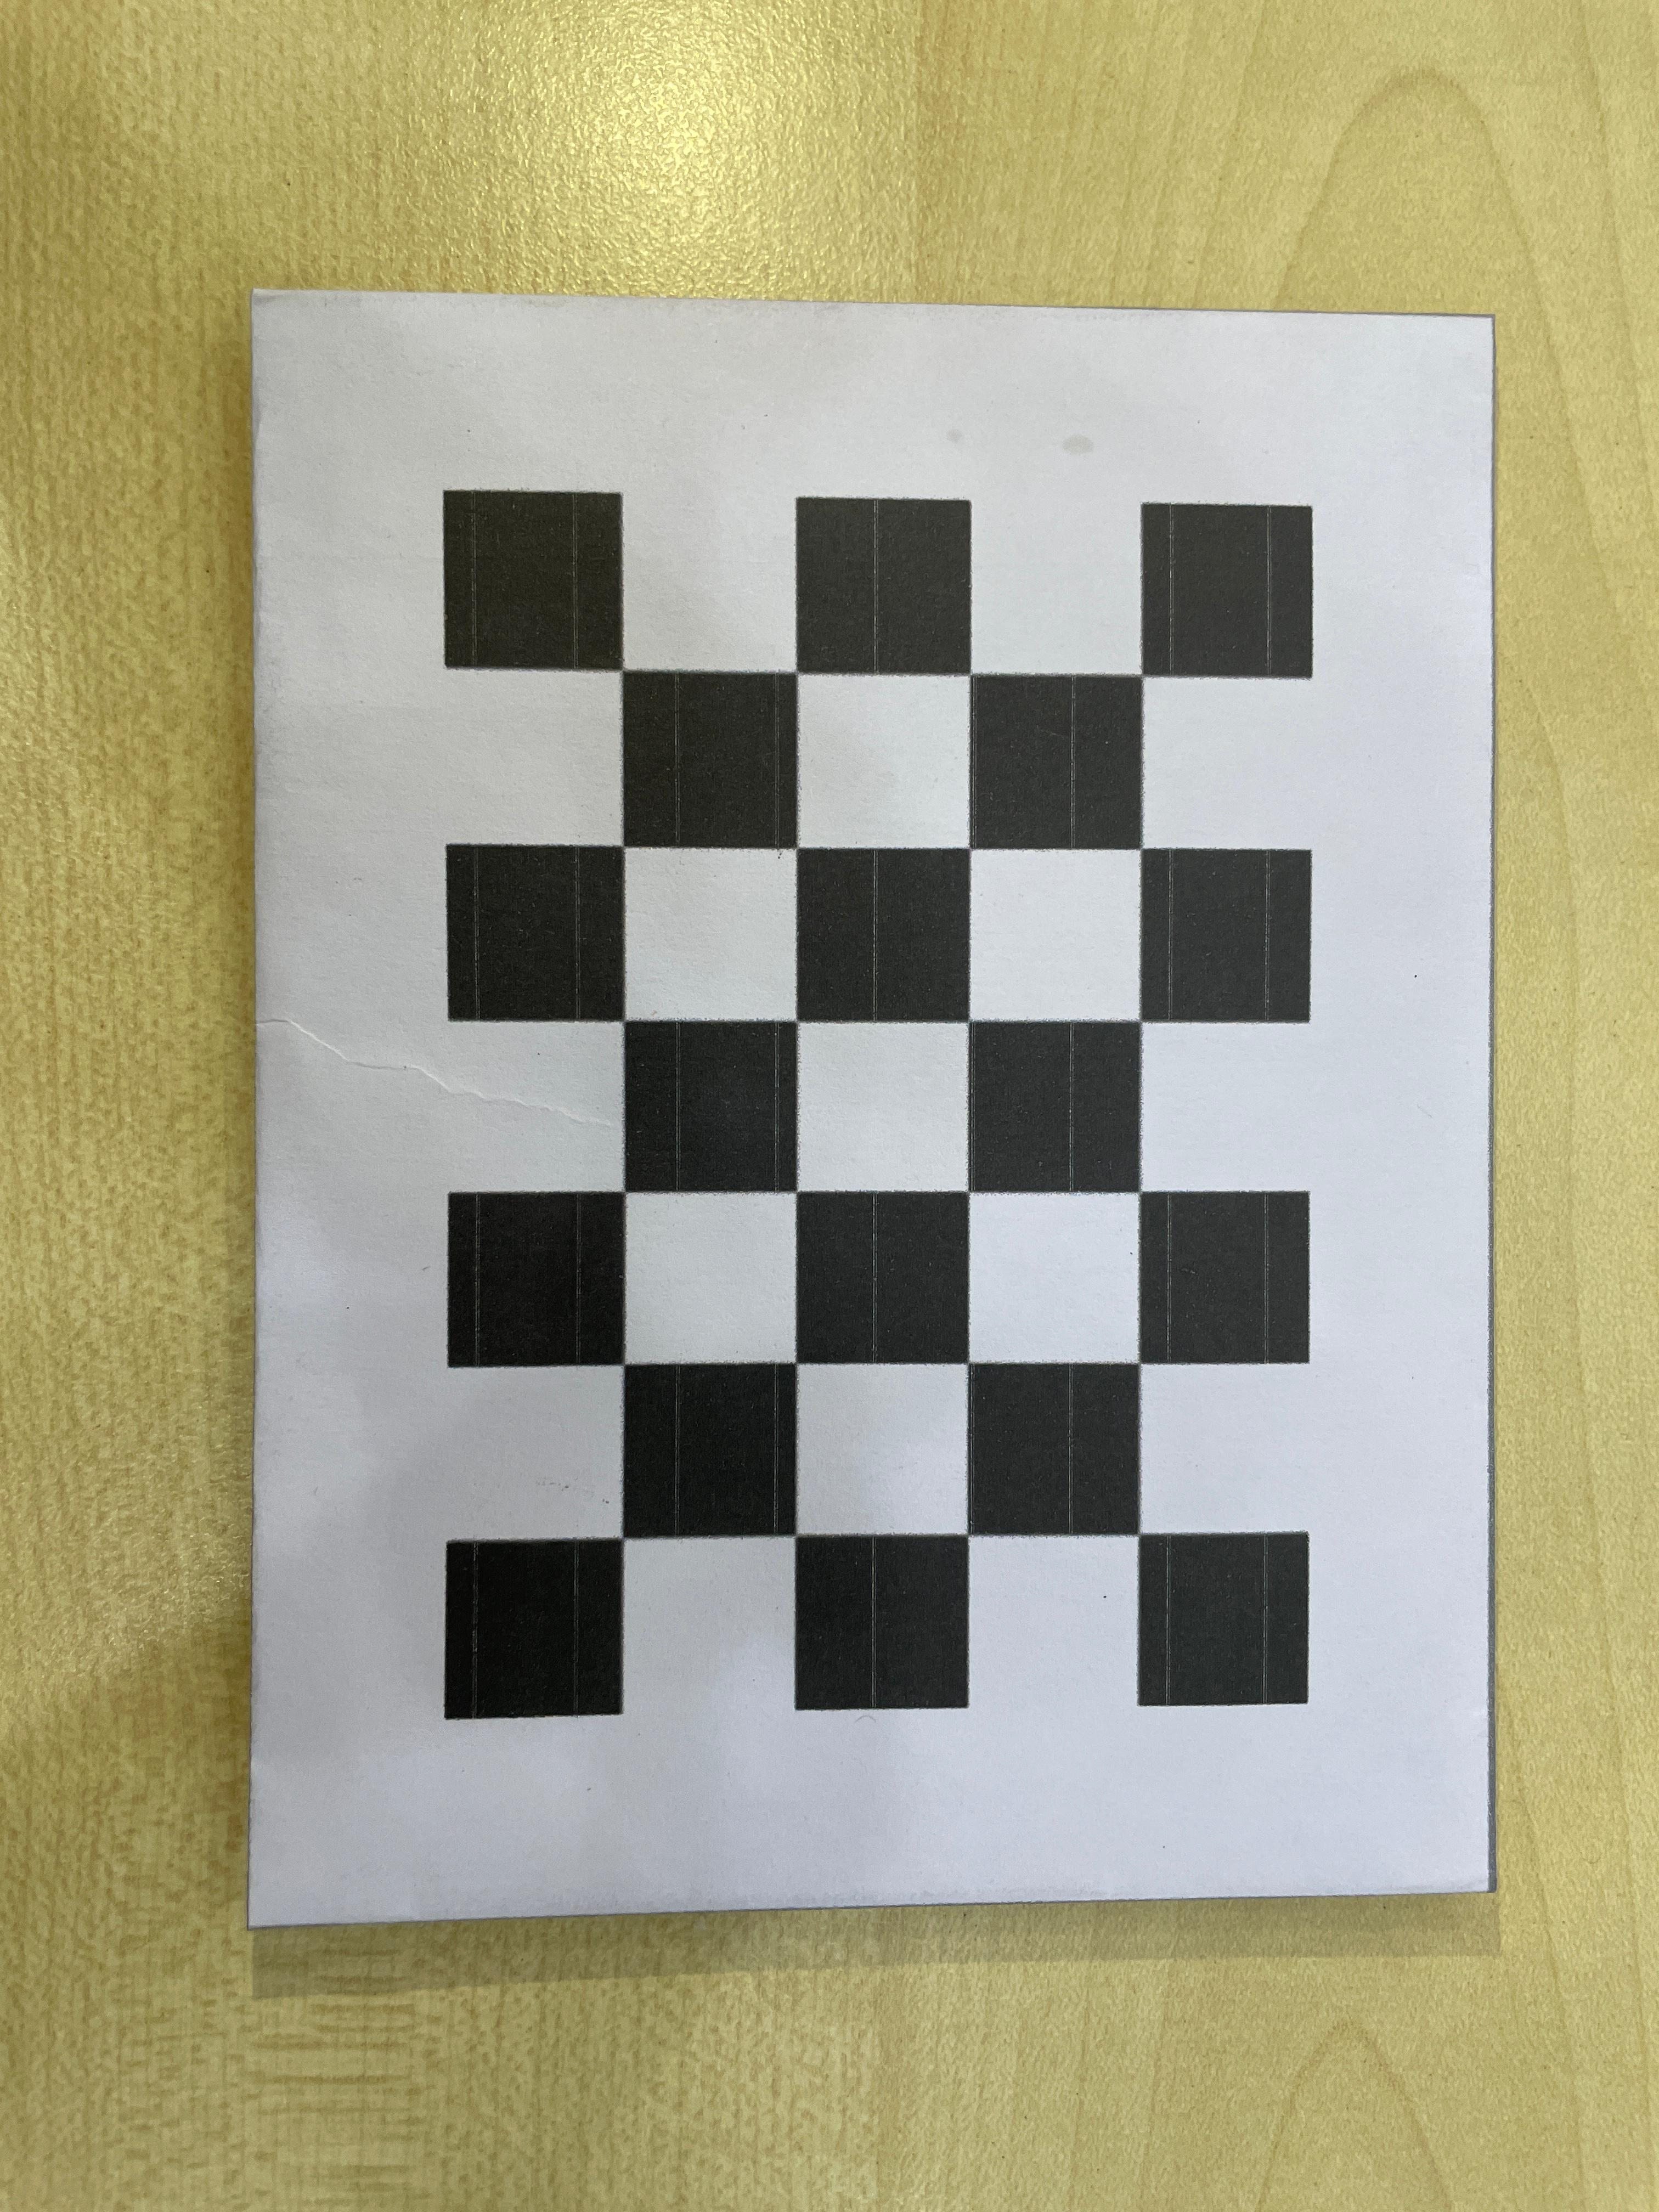
\includegraphics[width=0.075\textwidth, valign=c]{Assets/Camera-Calibration/01.jpg}
            & $\begin{bmatrix}
                1.0 & 0.0 & 0.0 \\
                0.0 & 1.0 & 0.0 \\
                0.0 & 0.0 & 1.0
            \end{bmatrix}$ & $\begin{bmatrix} -1.2 \\ -2.5 \\ 9.9 \end{bmatrix}$ \\
            & & \\
            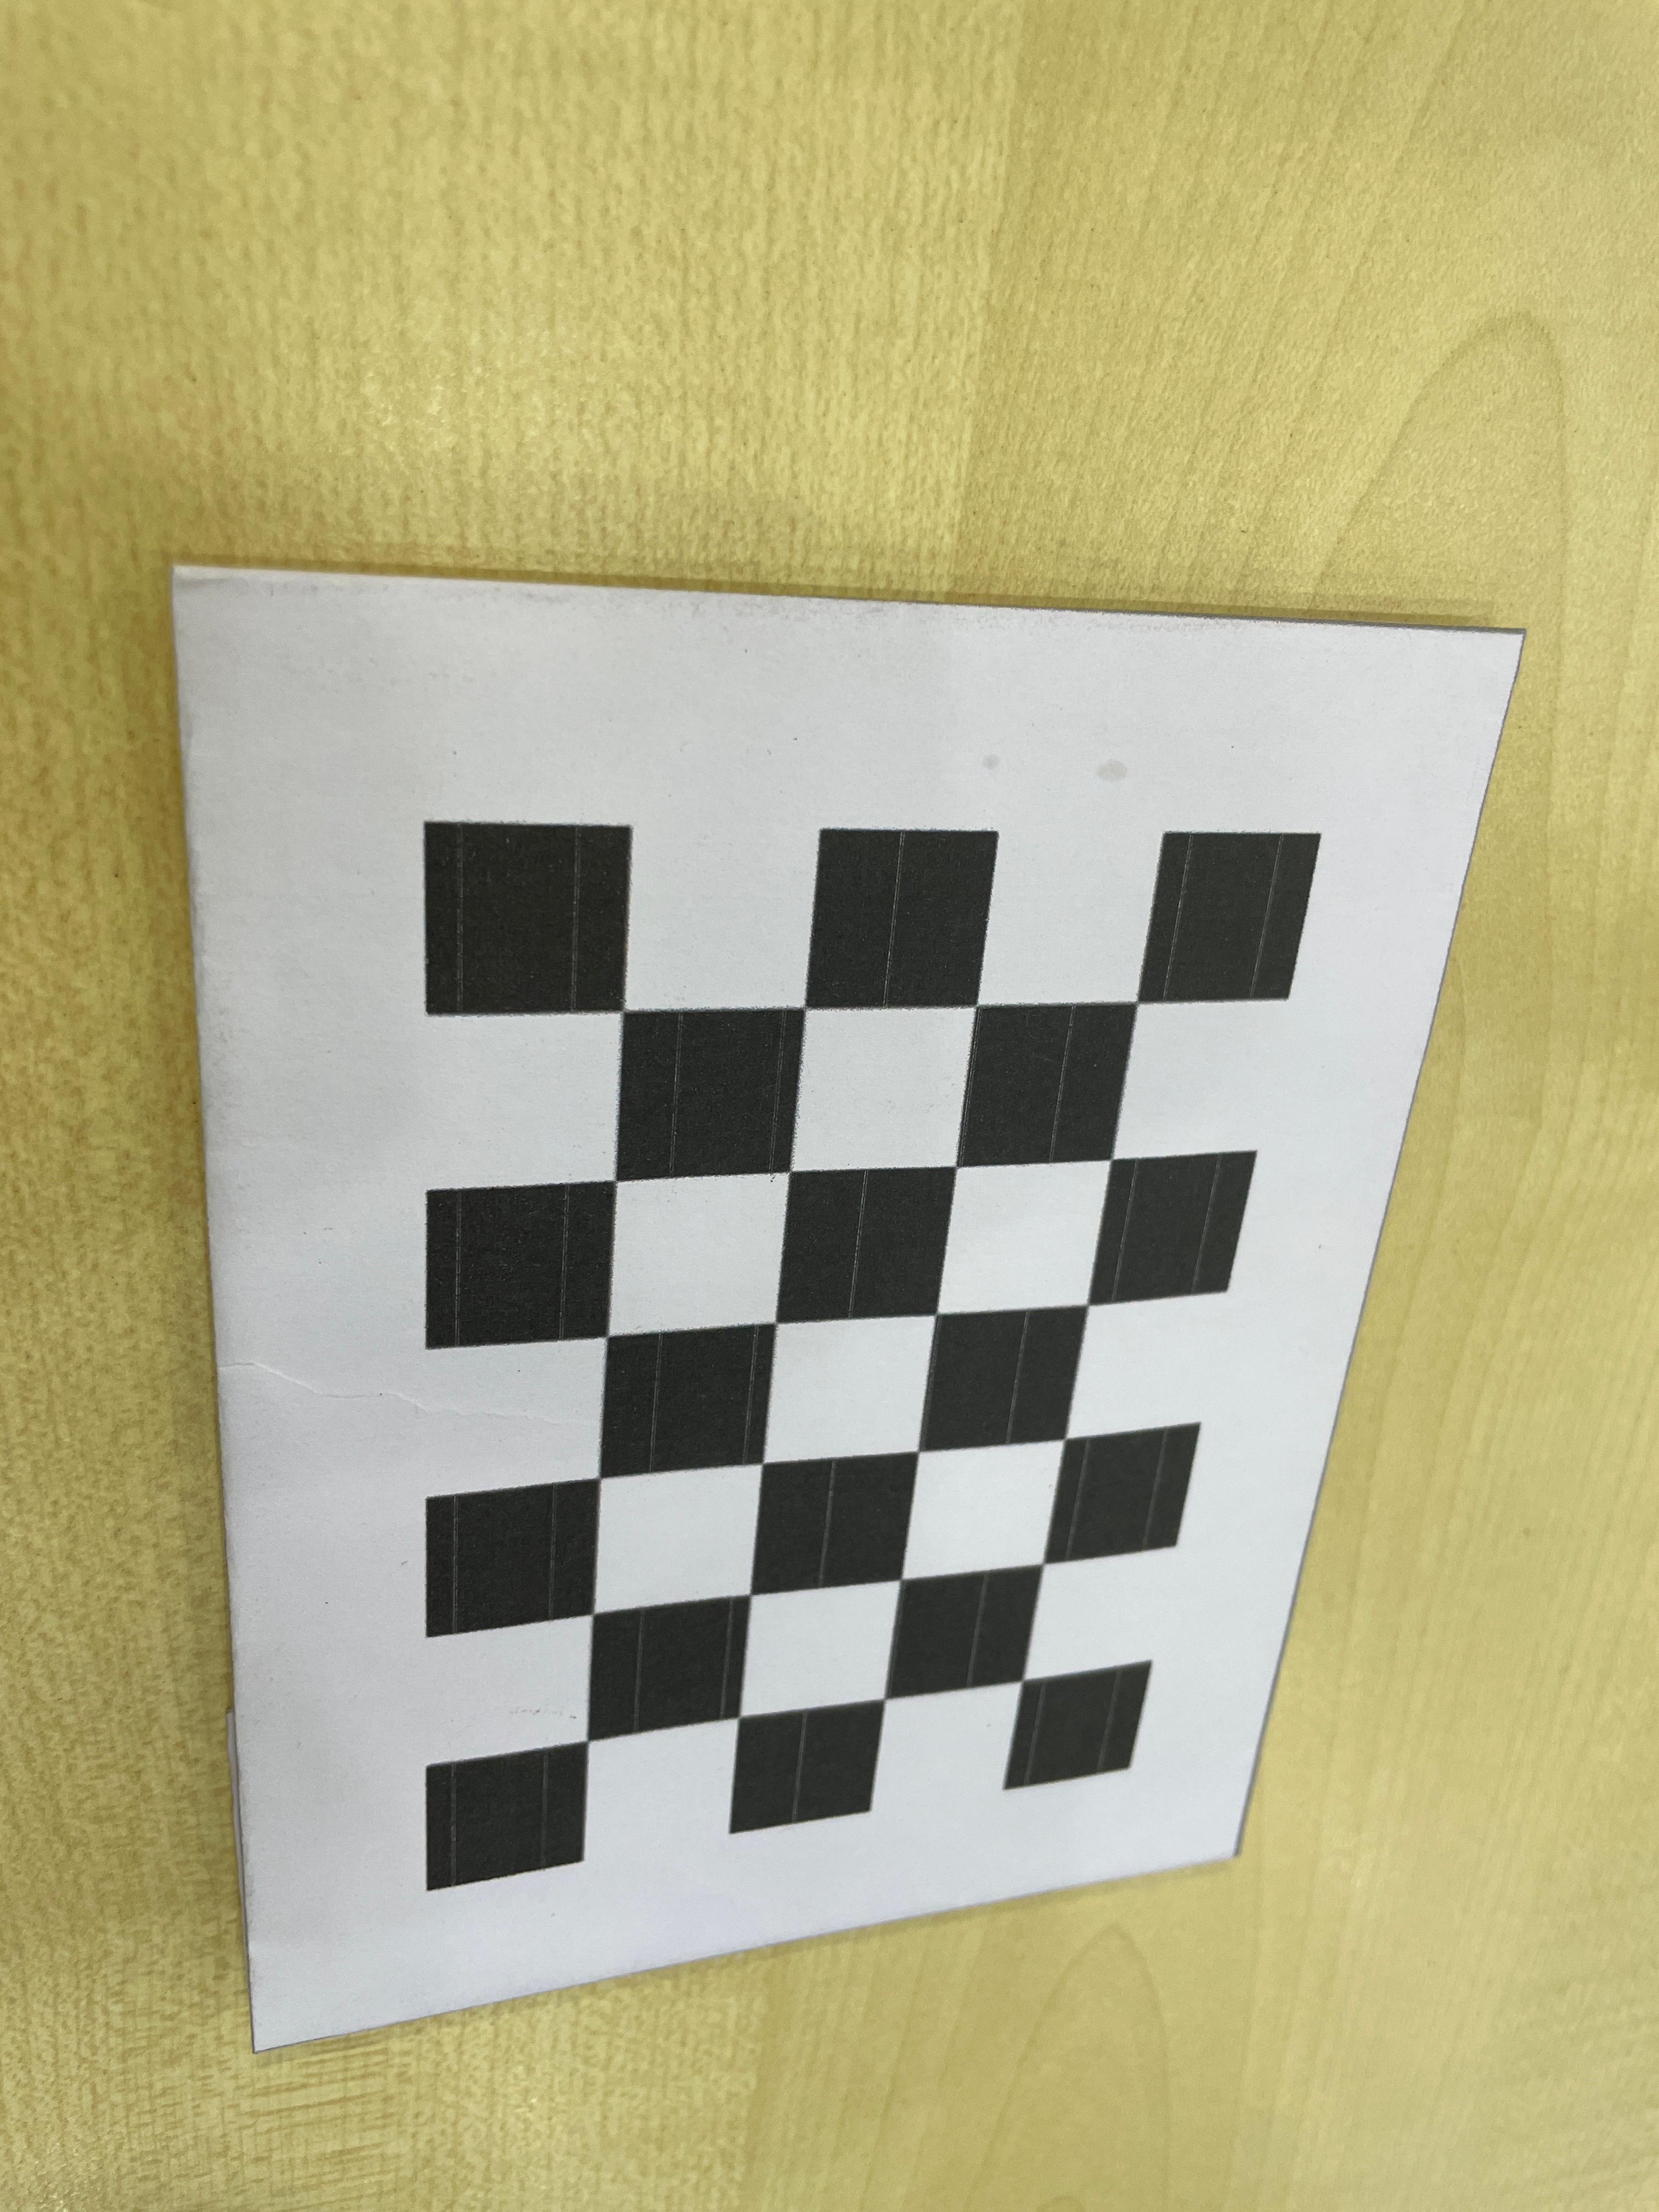
\includegraphics[width=0.075\textwidth, valign=c]{Assets/Camera-Calibration/02.jpg}
            & $\begin{bmatrix}
                0.9 & -0.1 & -0.3 \\
                0.1 & 0.9 & -0.4 \\
                0.3 & 0.4 & 0.8
            \end{bmatrix}$ & $\begin{bmatrix} -1.1 \\ -0.5 \\ 9.1 \end{bmatrix}$ \\
            & & \\
            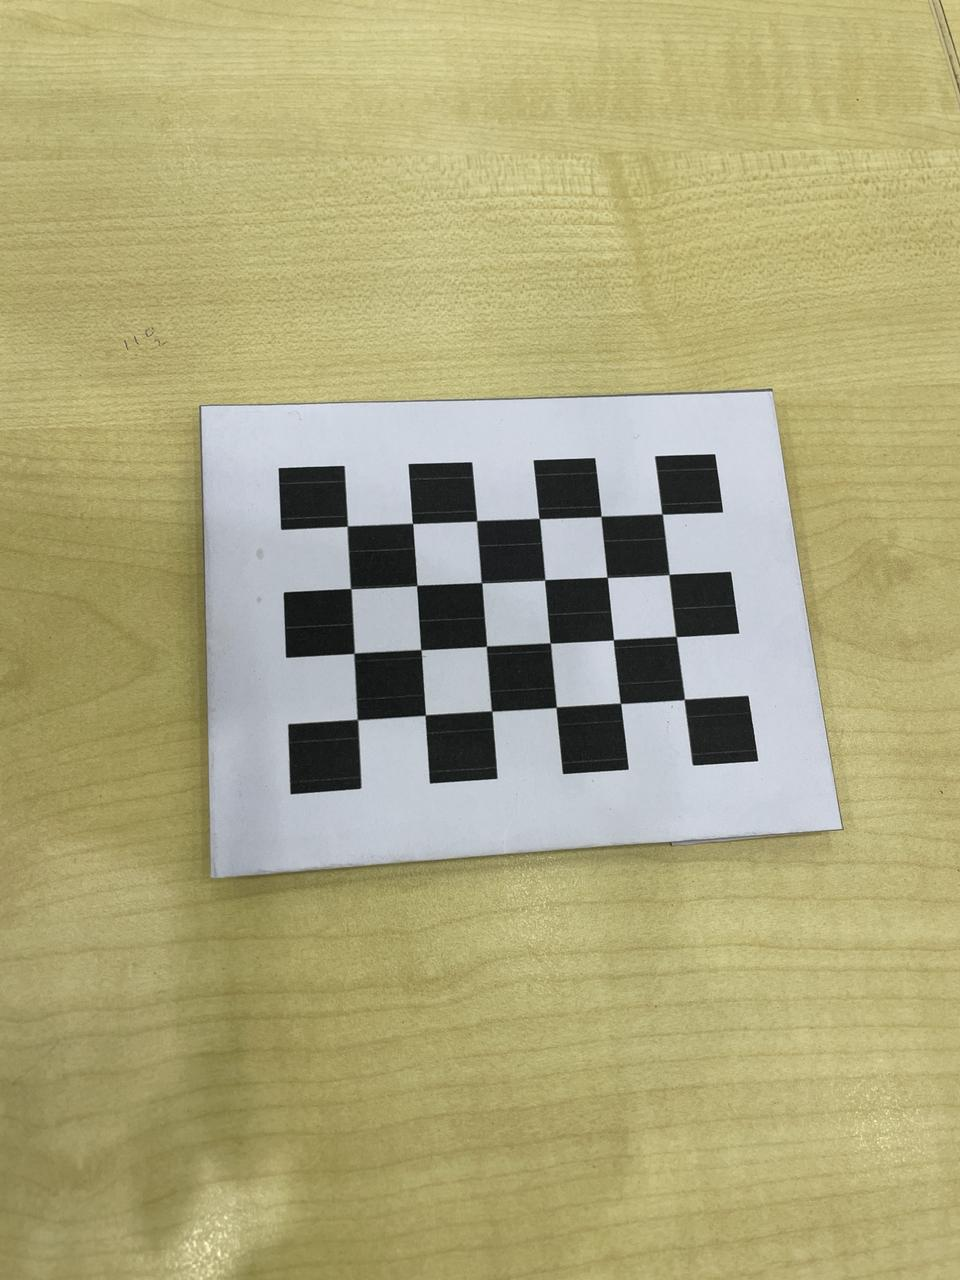
\includegraphics[width=0.075\textwidth, valign=c]{Assets/Camera-Calibration/03.jpg}
            & $\begin{bmatrix}
                0.1 & -0.9 & -0.4 \\
                0.9 & 0.2 & -0.2 \\
                0.2 & -0.3 & 0.9
            \end{bmatrix}$ & $\begin{bmatrix} -13.2 \\ -23.5 \\ 48.4 \end{bmatrix}$ \\
            & & \\
            \caption{Extrinsic camera parameters for the first three images}
            \label{tab:extrinsic-parameters}
        \end{longtable}

        \item We estimate the distortion parameters, specifically the tangenial and
        radial distortion parameters using the images. The following distortion vector
        was obtained.
        \begin{equation*}
            \mathbf{D} = \begin{bmatrix}
                k_{1} & k_{2} & p_{1} & p_{2} & k_{3}
            \end{bmatrix} = \begin{bmatrix}
                0.223 & -1.141 & -0.001 & -0.001 & 0.983
            \end{bmatrix}
        \end{equation*}
        indicating that the radial distortion coefficients are $k_{1} = 0.223$,
        $k_{2} = -1.141$, and $k_{3} = 0.983$. We then use these parameters to undisort
        5 images and compare the results with the original images. The comparison us given
        in \figref{distortions}.
        \begin{figure}[htbp]
            \begin{center}
                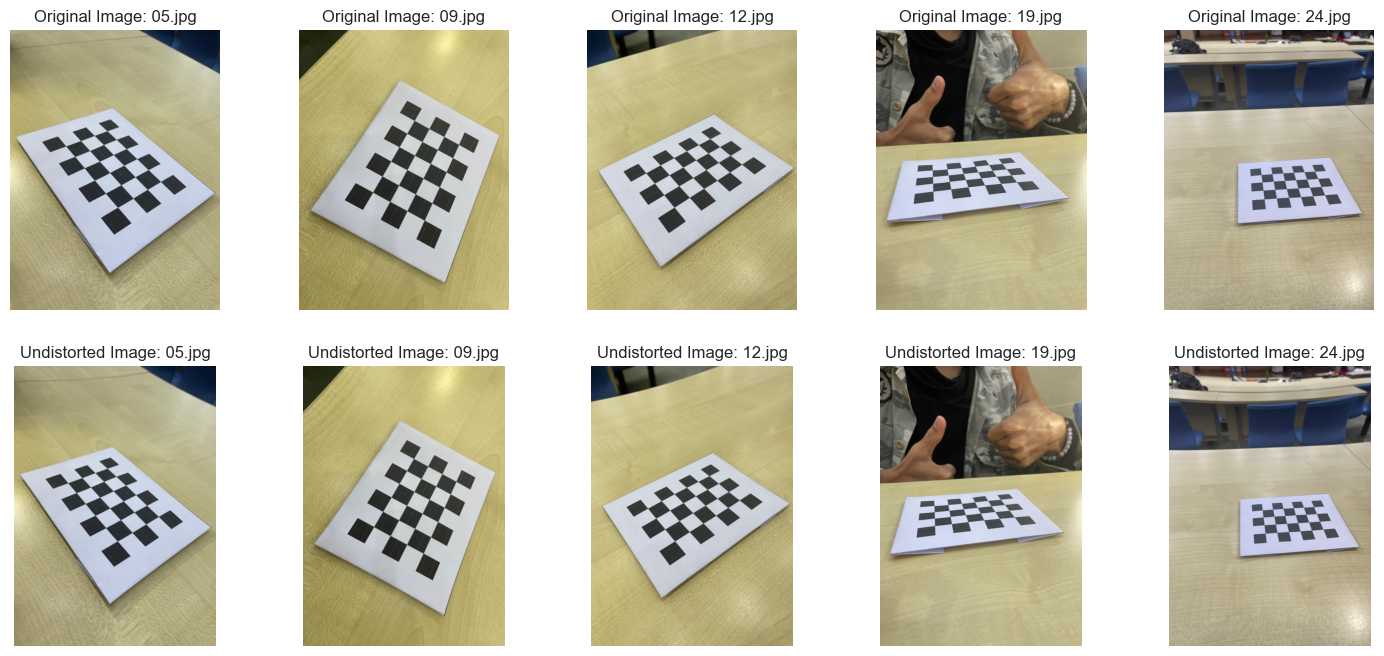
\includegraphics[width=0.875\textwidth]{Assets/Question-4/distortions.png}
                \caption{Comparison of 5 original and undisorted images}
                \label{fig:distortions}
            \end{center}
        \end{figure}
        \vspace*{0pt} \\
        We can see that on the edges/corners of the undisorted images, the straight lines
        appear to be curved; for example, in image 24, the edges of the tables behind the
        chessboard appear to be curved inward, i.e. showing negative curvature. Similar
        effects can be seen in image 9 and 12.

        \item We compute the reprojection error using the estimated intrinsic and extrinsic
        parameters of each of the 25 images. A bar chart of the reprojection errors is given
        in \figref{reprojection-error}.
        \begin{figure}[htbp]
            \begin{center}
                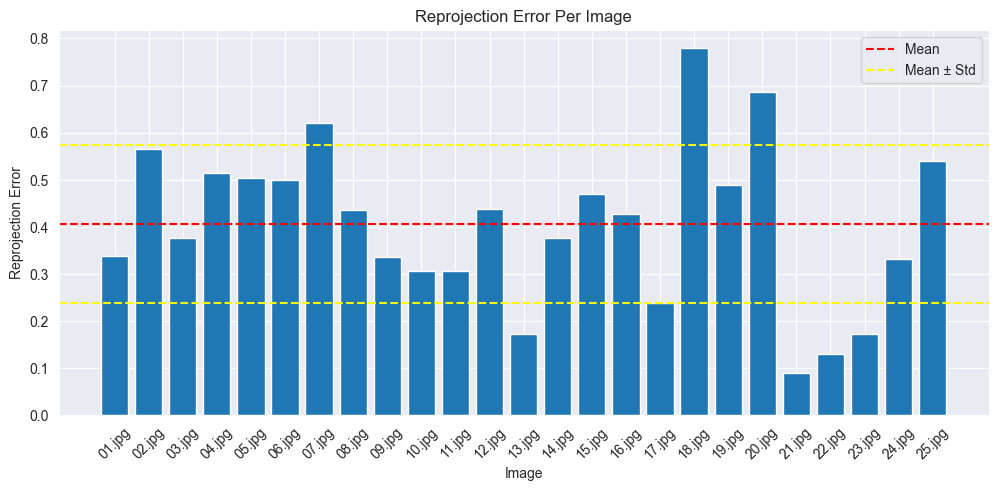
\includegraphics[width=0.875\textwidth]{Assets/Question-4/reprojection-error.png}
                \caption{Reprojection error for each of the 25 images}
                \label{fig:reprojection-error}
            \end{center}
        \end{figure}
        \vspace*{0pt} \\
        The mean reprojection error is $0.40$ pixels, with a standard deviation of $0.16$ pixels.

        \item We plot the figures of the chessboards showing the dettected corners and the
        corners after reprojecting them using the estimated intrinsic and extrinsic parameters.
        The figures are given in \figref{corners}. In the figure, the red crosses are the
        detected corners, while the blue circles are the reprojected corners. The images are
        ordered as before.
        \begin{figure}[htbp]
            \begin{center}
                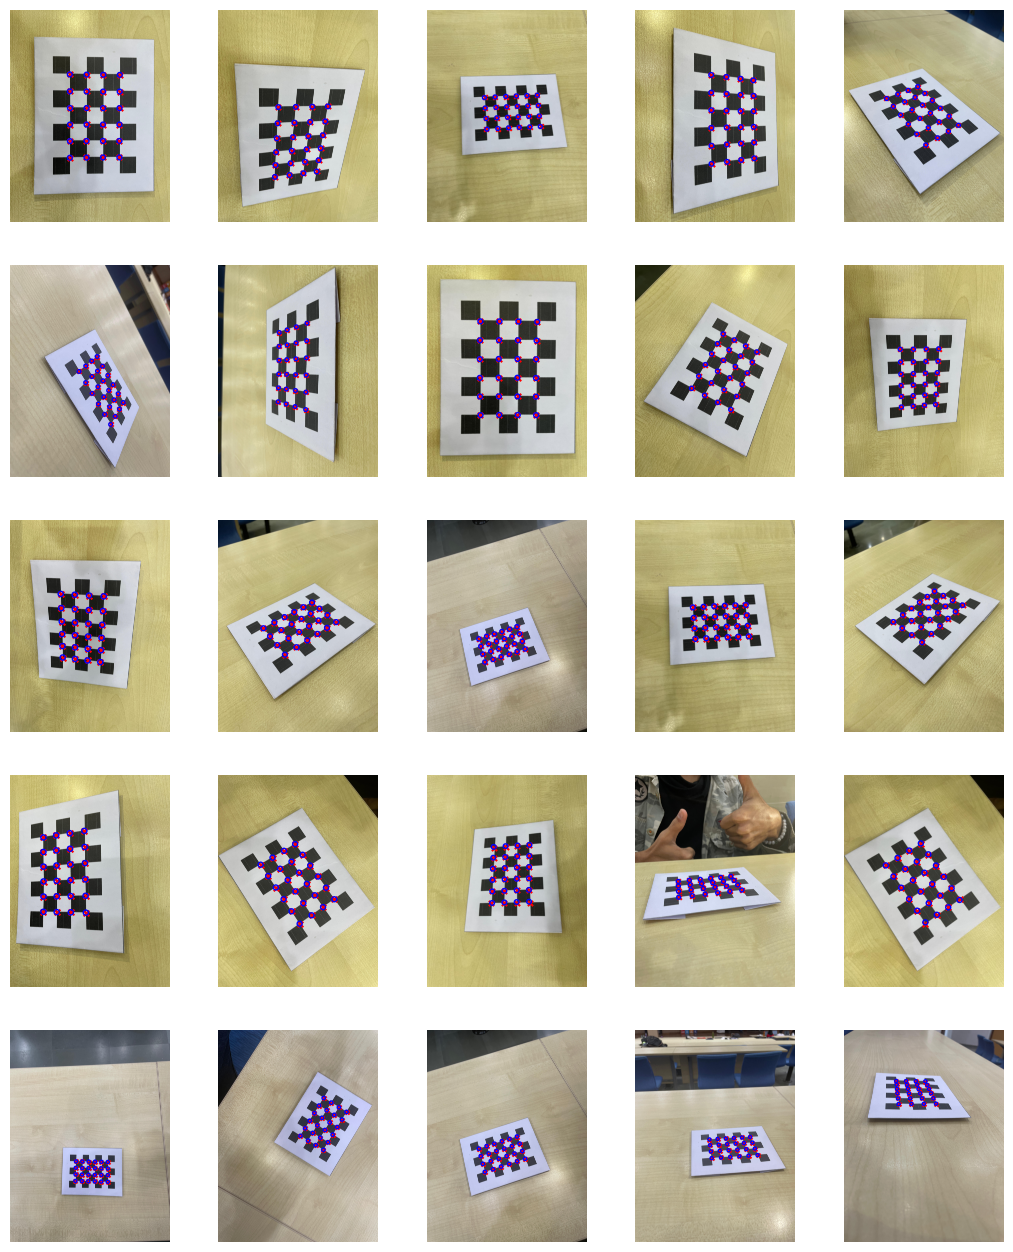
\includegraphics[width=0.875\textwidth]{Assets/Question-4/corners.png}
                \caption{Detected and reprojected corners of the chessboard}
                \label{fig:corners}
            \end{center}
        \end{figure}
        Reprojection error is computed as the average of the Euclidean distances between the
        detected and reprojected corners, i.e.
        \begin{equation*}
            \mathbf{e}(\mathbf{c}, \mathbf{c'}) =
            \frac{1}{N} \sum_{i=1}^{N} \left\| \mathbf{c}_{i} - \mathbf{c'}_{i} \right\|_{2}
        \end{equation*}
        where $\mathbf{c}_{i}$ and $\mathbf{c'}_{i}$ are the observed and reprojected
        2D coordinates of the $i$-th corner, and $N$ is the number of corners.

        \item We compute the chessboard plane normals $\mathbf{\hat{n}}_{i}^{C}$ in the
        camera coordinate frame for each image. The normals are given in Table
        \ref{tab:plane-normals}. The figures are rounded off to two decimal places for
        brevity. The precise parameters for each image can be found in the notebook.
        \begin{longtable}{c|c}
            \textsc{Image} & \textsc{Plane Normal} \\
            \hline & \\
            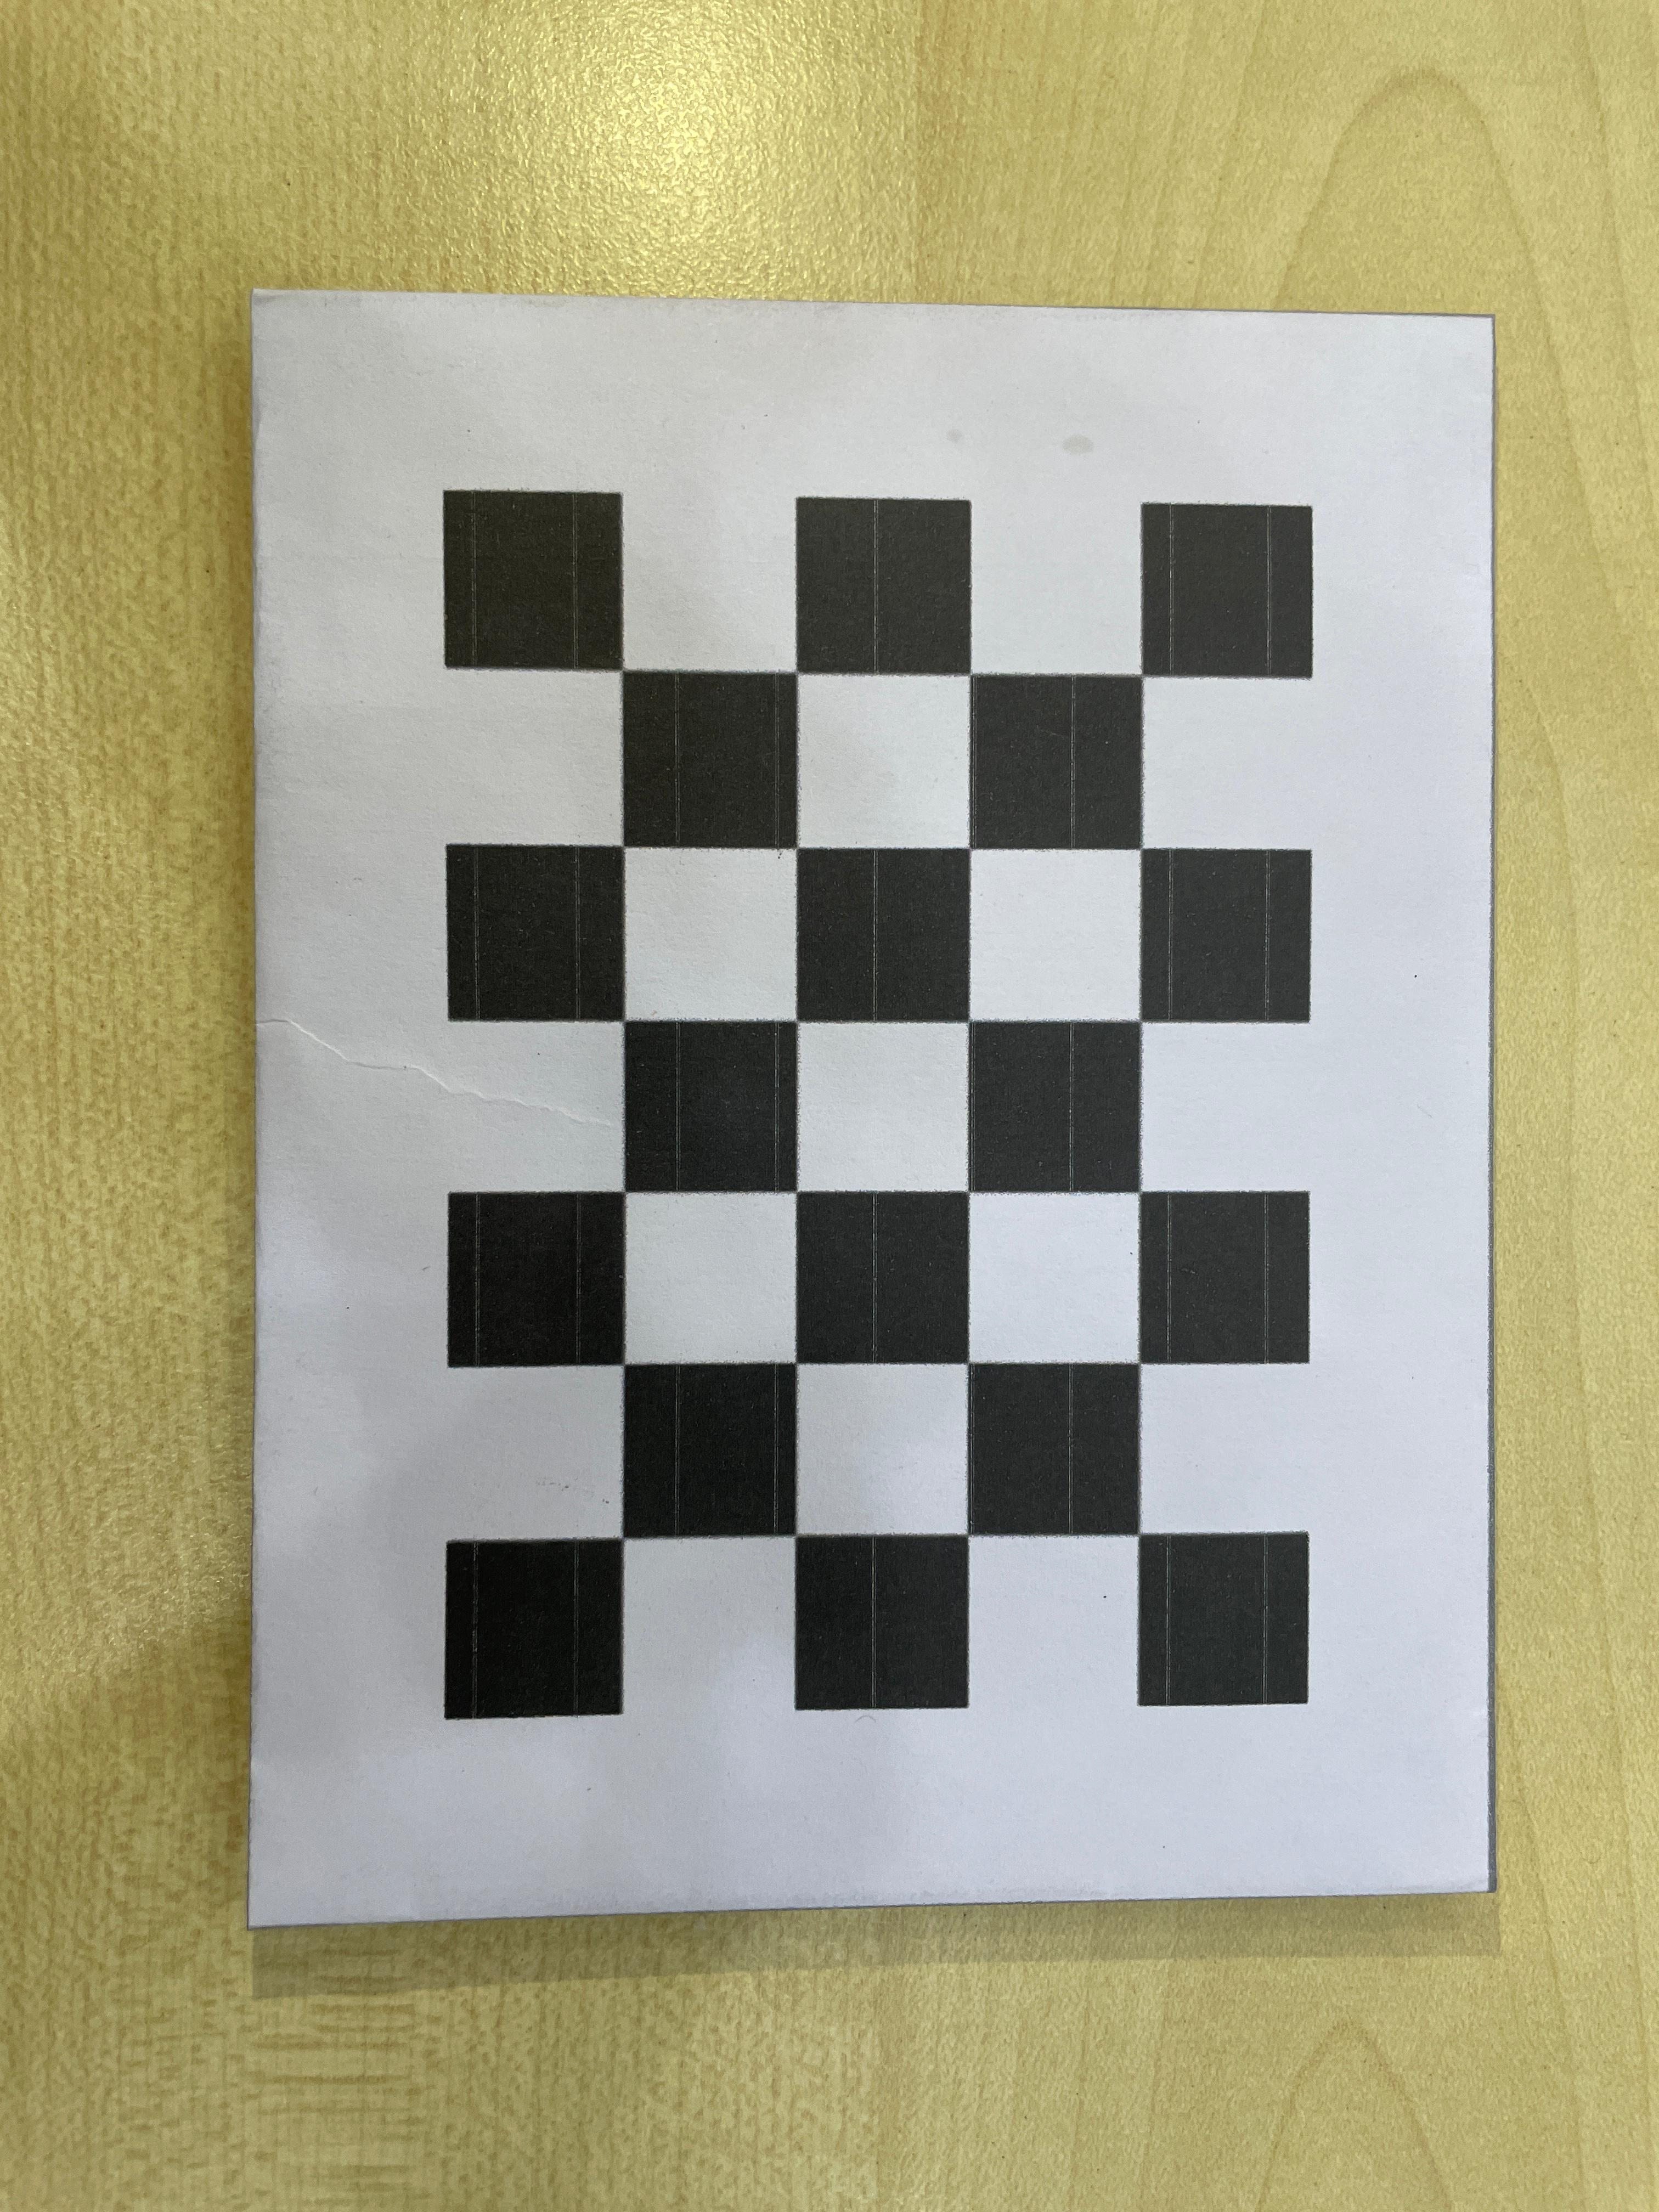
\includegraphics[width=0.075\textwidth, valign=c]{Assets/Camera-Calibration/01.jpg}
            & $\begin{bmatrix} -0.03 & -0.01 & 0.99 \end{bmatrix}^{\top}$ \\
            & \\
            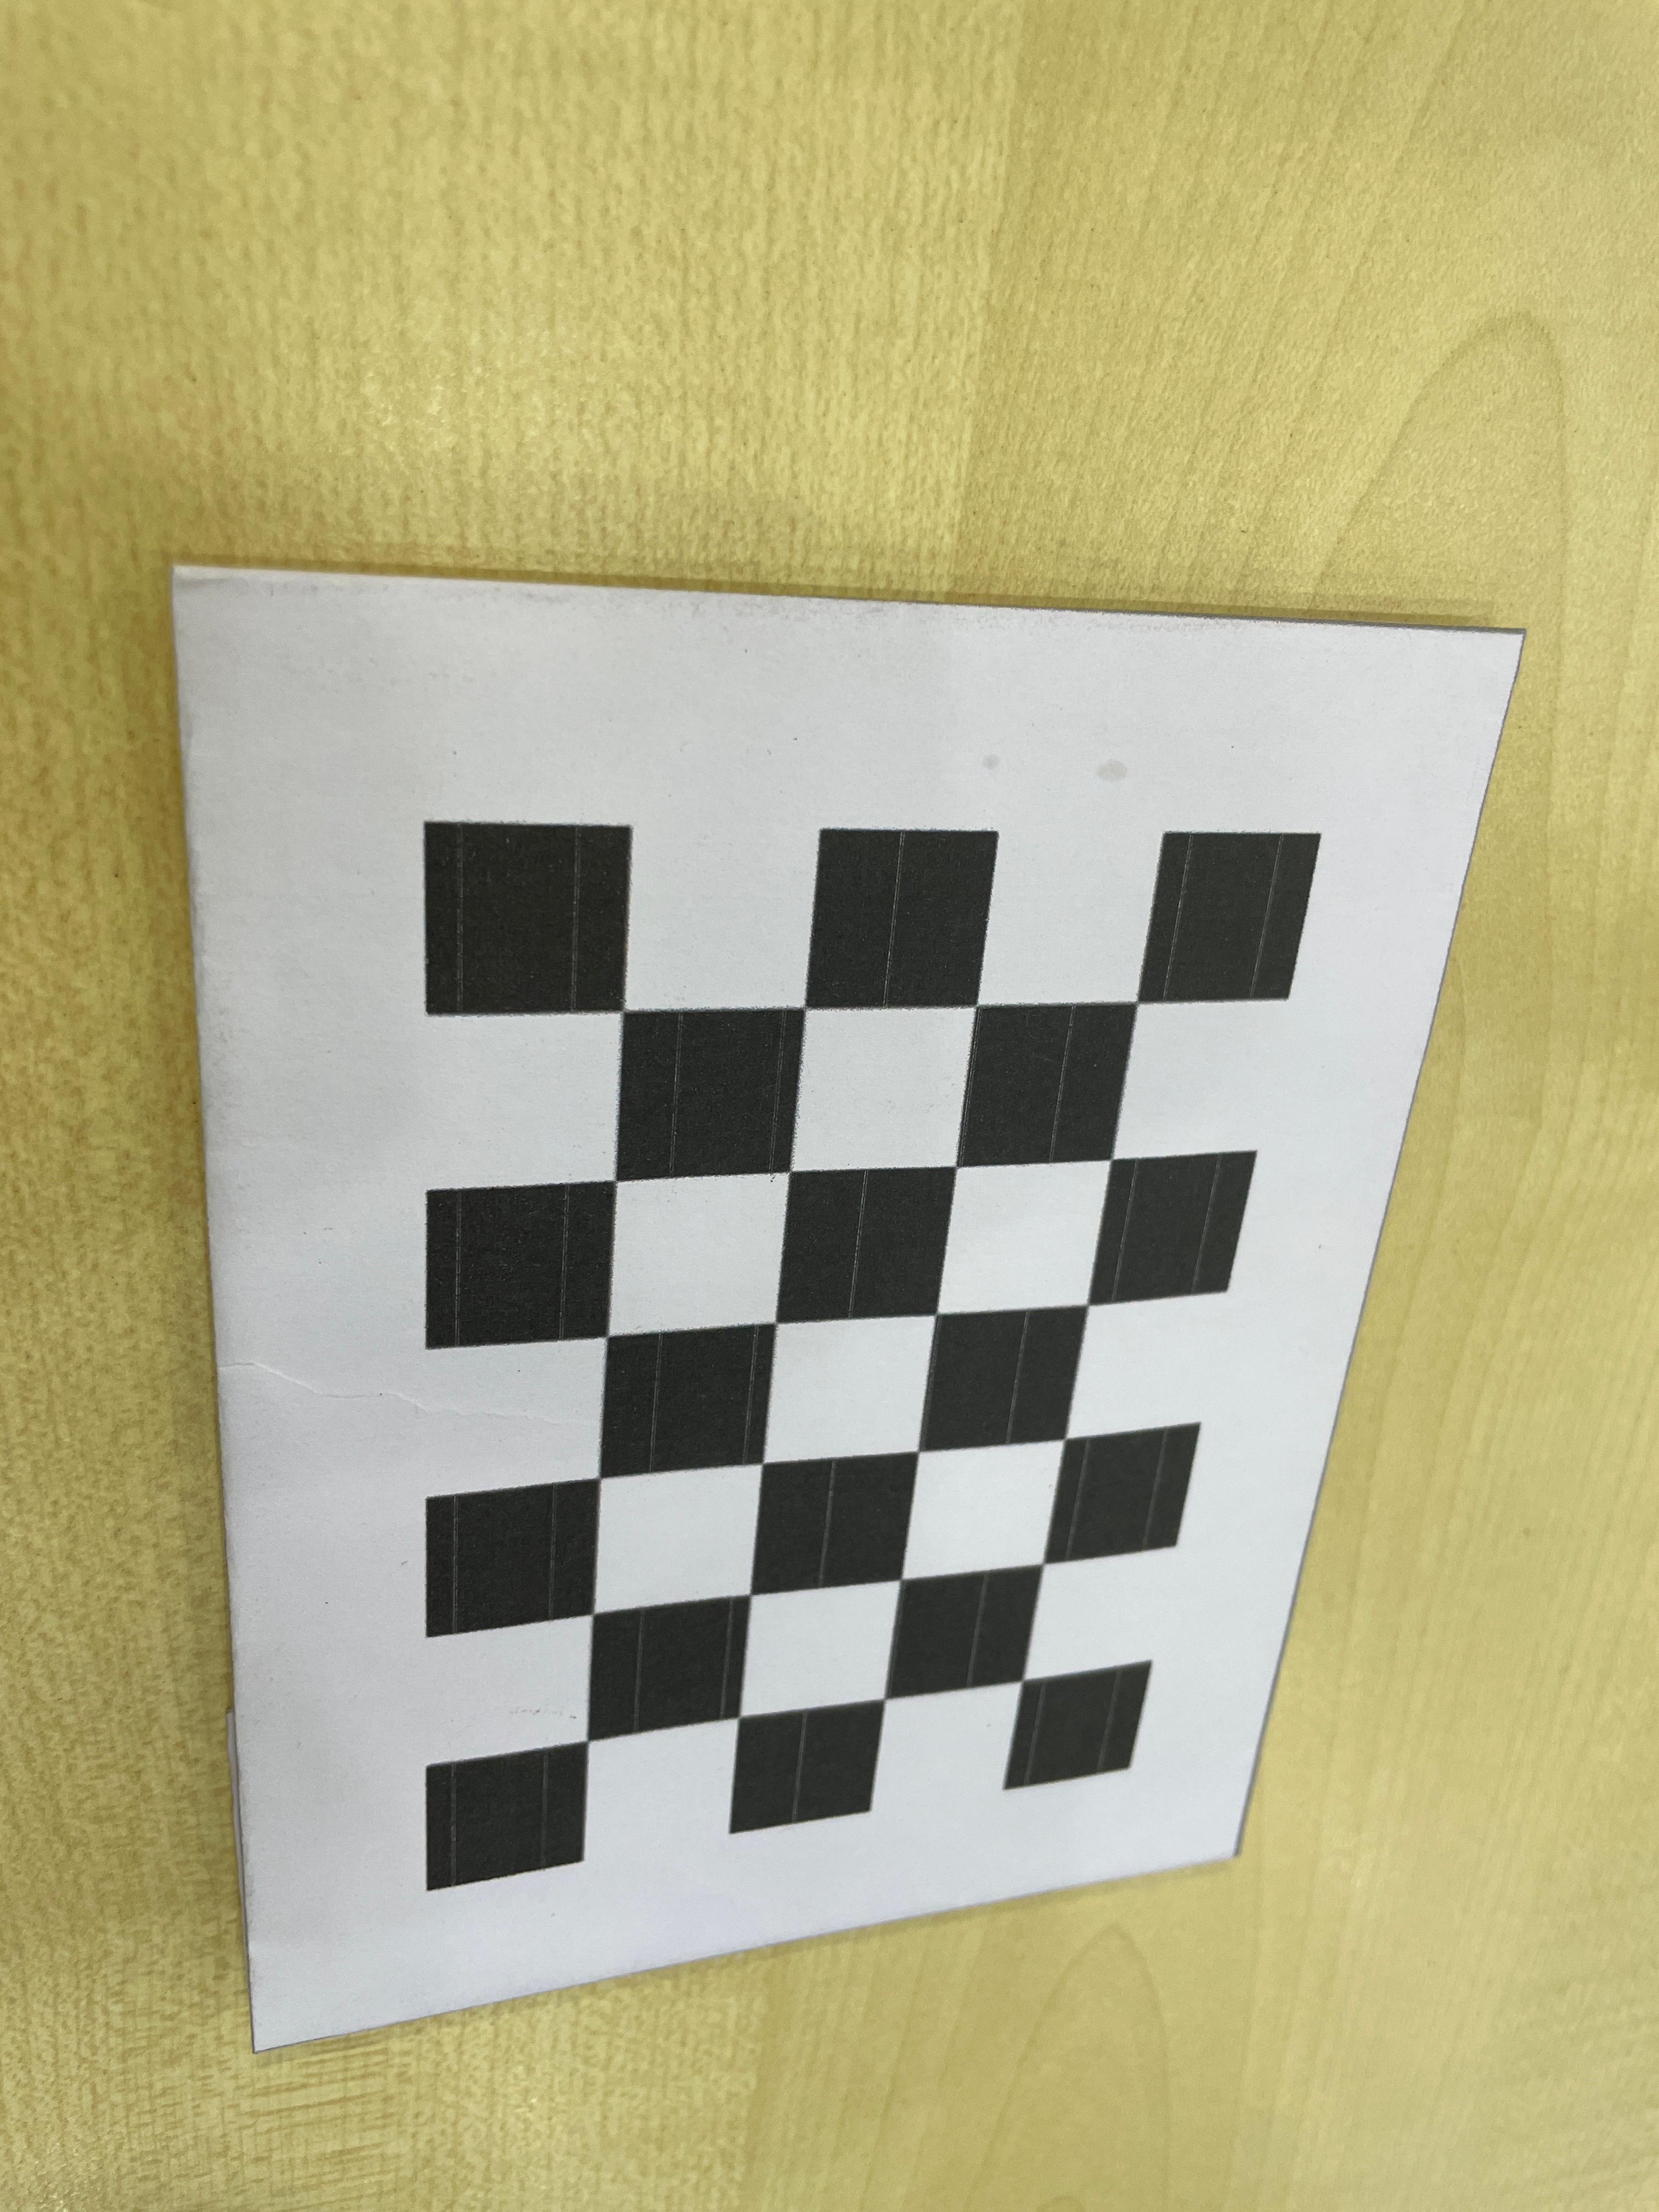
\includegraphics[width=0.075\textwidth, valign=c]{Assets/Camera-Calibration/02.jpg}
            & $\begin{bmatrix} -0.27 & -0.40 & 0.87 \end{bmatrix}^{\top}$ \\
            & \\
            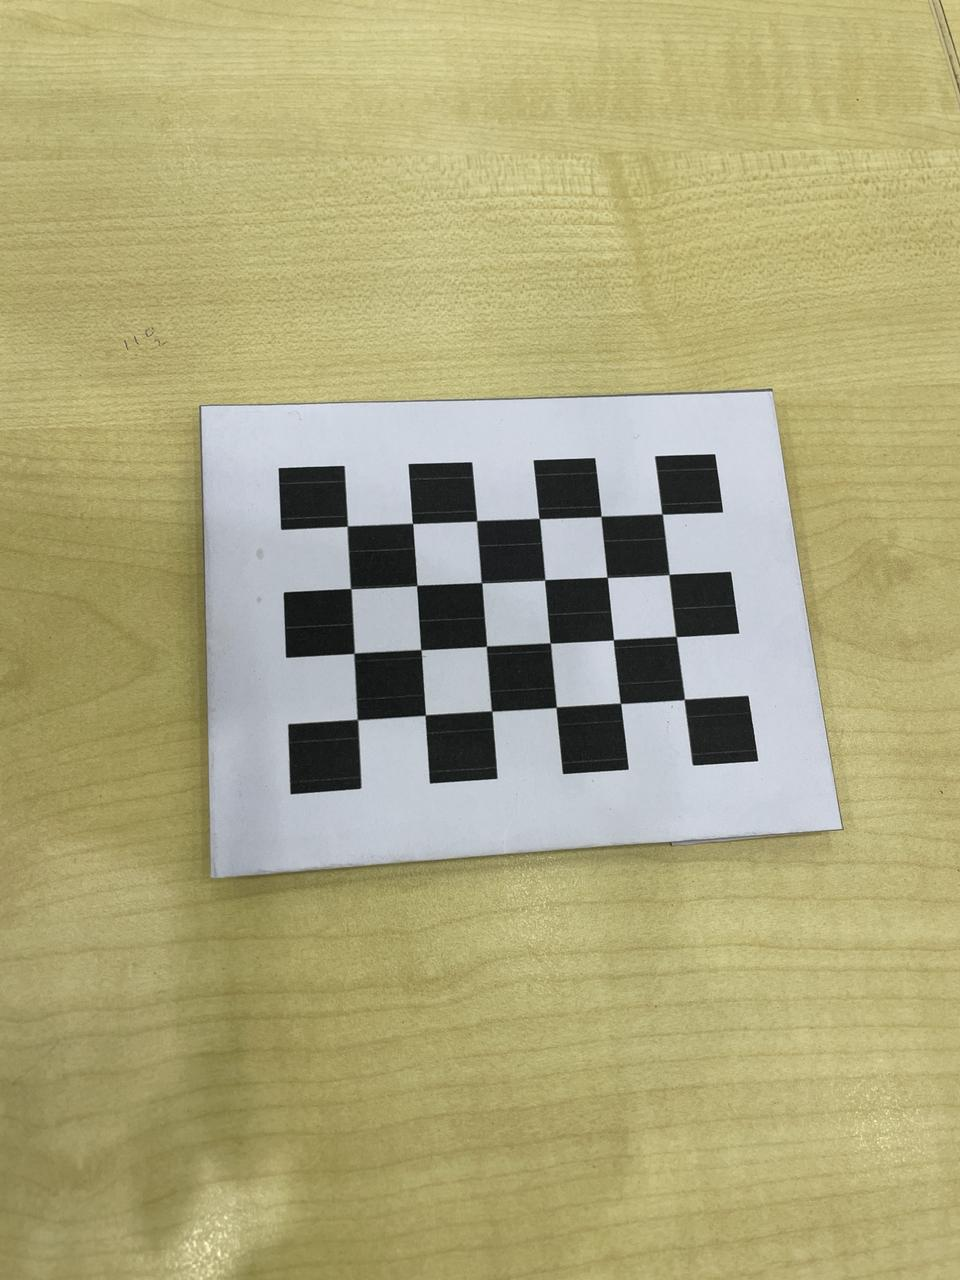
\includegraphics[width=0.075\textwidth, valign=c]{Assets/Camera-Calibration/03.jpg}
            & $\begin{bmatrix} -0.42 & -0.16 & 0.89 \end{bmatrix}^{\top}$ \\
            & \\
            \caption{Plane normals for the first three images}
            \label{tab:plane-normals}
        \end{longtable}
        As opposed to just numbers, we can visualize the normals on the chessboard. This
        was done by projecting the normal to the chessboard on the image. The figures are
        given in \figref{normals}. The normals are shown as red lines on the chessboard,
        while the green diagonals indicate the chessboard plane.
        \begin{figure}[htbp]
            \begin{center}
                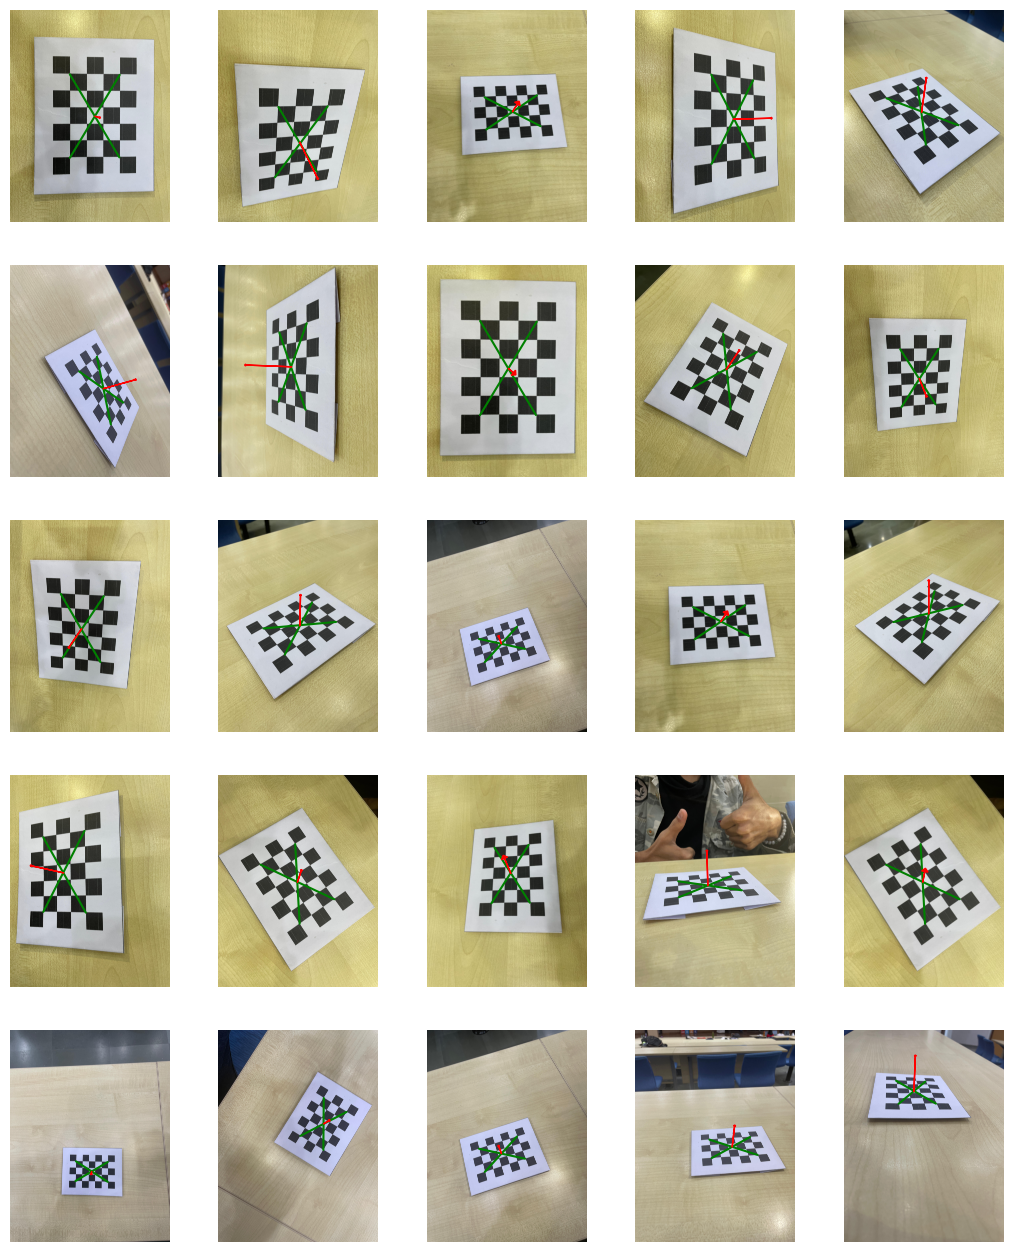
\includegraphics[width=0.875\textwidth]{Assets/Question-4/normals.png}
                \caption{Plane normals for each of the 25 images}
                \label{fig:normals}
            \end{center}
        \end{figure}
    \end{enumerate}
    \pagebreak

    \section*{\textbf{Question 5. (Camera-LIDAR Cross-Calibration)}}
    We are required to perform Camera-LIDAR Cross-Calibration with the given set of
    images and their corresponding LIDAR scans. From the given dataset, we choose a
    set of 25 images to perform the cross-calibration, which are given in
    \figref{final-lidar-set}. The code for this question is given in
    \texttt{LIDAR-cross-calibration.ipynb}.
    \begin{figure}[htbp]
        \begin{center}
            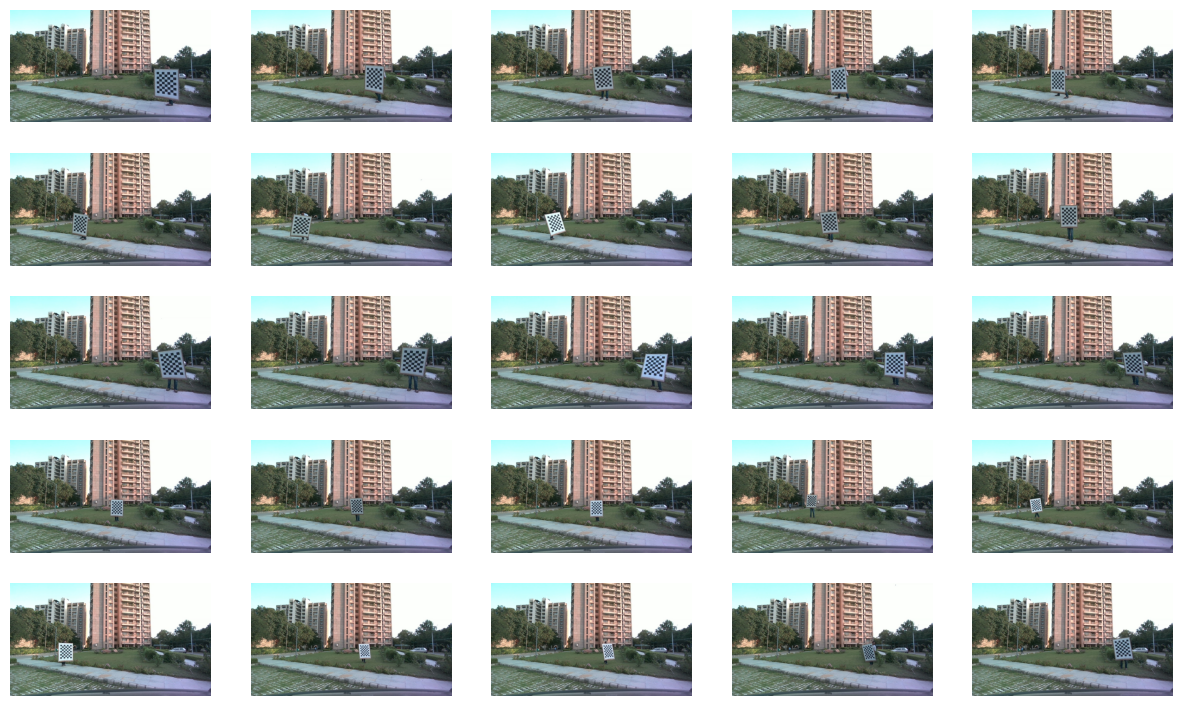
\includegraphics[width=0.875\textwidth]{Assets/Question-5/final-image-set.png}
            \caption{Images used for camera-LIDAR cross-calibration}
            \label{fig:final-lidar-set}
        \end{center}
    \end{figure}
    \begin{enumerate}
        \item We first compute the chessboard plane normals $\mathbf{\hat{n}}_{i}^{L}$ in
        in the LIDAR coordinate frame using the points given in the \texttt{.pcd} files
        and their corresponding offsets. We calculate the normals using singular value
        decomposition (SVD) of the matrix of points as follows. For the $i^{th}$ scan, let
        \begin{equation*}
            X_{N \times 3}^{(i)} = \begin{bmatrix}
                \mathbf{x}_{1}^{(i)} & \mathbf{x}_{2}^{(i)} & \cdots & \mathbf{x}_{N}^{i}
            \end{bmatrix}^{\top}
        \end{equation*}
        be the matrix of points in the LIDAR coordinate frame, where each
        $\mathbf{x}_{j}^{(i)}$ is a 3D point and $N$ is the number of points. Then, the
        normal $\mathbf{\hat{n}}_{i}^{L}$ to the plane of the points is given by the
        rightmost column of the matrix $V$ where
        \begin{equation*}
            X^{(i)} - \mathbf{\bar{x}}^{(i)} = U \Sigma V^{\top}
        \end{equation*}
        is the singular value decomposition of the matrix of centered points
        $X^{(i)} - \mathbf{\bar{x}}^{(i)}$, where $\mathbf{\bar{x}}^{(i)}$ is the centroid
        or mean of the points. The offset is simply
        \begin{equation*}
            \theta_{i} = \mathbf{\hat{n}}_{i}^{L} \cdot \mathbf{\bar{x}}^{(i)}
        \end{equation*}
        which is the scalar in the equation of the plane. In case the offset is negative,
        we negate the normal and the offset. The normals and offsets for the first three
        scans are given in Table \ref{tab:lidar-normals}. The figures are rounded off to
        two decimal places for brevity. The precise parameters for each scan can be found
        in the notebook.
        \begin{longtable}{c|c|c}
            \textsc{Scan} & \textsc{Plane Normal} & \textsc{Offset} \\
            \hline & & \\
            \includegraphics[width=0.2\textwidth, valign=c]{../Datasets/LIDAR/camera_images/frame_1061.jpeg}
            & $\begin{bmatrix} 0.64 & -0.77 & 0.1 \end{bmatrix}^{\top}$ & $5.0$ \\
            & & \\
            \includegraphics[width=0.2\textwidth, valign=c]{../Datasets/LIDAR/camera_images/frame_1075.jpeg}
            & $\begin{bmatrix} 0.7 & -0.7 & 0.12 \end{bmatrix}^{\top}$ & $4.72$ \\
            & & \\
            \includegraphics[width=0.2\textwidth, valign=c]{../Datasets/LIDAR/camera_images/frame_1093.jpeg}
            & $\begin{bmatrix} 0.94 & -0.23 & 0.26 \end{bmatrix}^{\top}$ & $5.2$ \\
            & & \\
            \caption{Plane normals and offsets for the first three LIDAR scans}
            \label{tab:lidar-normals}
        \end{longtable}

        \item Now we derive the equations.

        \item Using the above equations, we estimate the LIDAR-to-Camera transformation
        matrix. Using the closed form solution given in the thesis [2], if
        \begin{equation*}
            \mathbf{n}_{C} = \begin{bmatrix}
                \hat{\mathbf{n}}_{1}^{(C)} \\ \hat{\mathbf{n}}_{2}^{(C)} \\ \vdots \\ \hat{\mathbf{n}}_{N}^{(C)}
            \end{bmatrix}_{N \times 3} \quad
            \mathbf{n}_{L} = \begin{bmatrix}
                \hat{\mathbf{n}}_{1}^{(L)} \\ \hat{\mathbf{n}}_{2}^{(L)} \\ \vdots \\ \hat{\mathbf{n}}_{N}^{(L)}
            \end{bmatrix}_{N \times 3} \quad
            \mathbf{d}_{C} = \begin{bmatrix}
                d_{1}^{(C)} \\ d_{2}^{(C)} \\ \vdots \\ d_{N}^{(C)}
            \end{bmatrix}_{N \times 1} \quad
            \mathbf{d}_{L} = \begin{bmatrix}
                d_{1}^{(L)} \\ d_{2}^{(L)} \\ \vdots \\ d_{N}^{(L)}
            \end{bmatrix}_{N \times 1}
        \end{equation*}
        then
        \begin{align*}
            ^{C} t_{L} &= (\mathbf{n}_{C}^{\top} \mathbf{n}_{C})^{-1} \mathbf{n}_{C}^{\top} (d_{C} - d_{L}) \\
            ^{C} \mathbf{R}_{L} &= V U^{\top} \quad \text{if} \quad
            \mathbf{n}_{L}^{\top} \mathbf{n}_{C} = U \Sigma V^{\top}
        \end{align*}
        where $\mathbf{n}_{C}$ and $\mathbf{n}_{L}$ are the matrices of normals in the
        camera and LIDAR coordinate frames, $N$ is the number of points, $\mathbf{d}_{C}$
        and $\mathbf{d}_{L}$ are the vectors of offsets in the camera and LIDAR coordinate
        frames, and $U$, $\Sigma$, and $V$ are the matrices obtained from the singular
        value decomposition of $\mathbf{n}_{L}^{\top} \mathbf{n}_{C}$. Then, the
        transformation matrix is simply
        \begin{equation*}
            ^{C} \mathbf{\tilde{T}}_{L} = \begin{bmatrix} ^{C}
                \mathbf{R}_{L} \mid \ ^{C} t_{L}
            \end{bmatrix}_{4 \times 3}
        \end{equation*}
        The above closed form solution was implemented in the notebook to estimate the
        transformation matrix. The following transformation matrix was obtained
        (rounded off to two decimal places for brevity).
        \begin{equation*}
            ^{C} \mathbf{\tilde{T}}_{L} = \begin{bmatrix}
                -0.18 & -0.98 & 0.0 & 0.15 \\
                0.02 & 0.0 & -0.99 & -0.41 \\
                0.98 & -0.18 & 0.02 & -0.6
            \end{bmatrix}
        \end{equation*}
        It can be noted that the determinant of the rotation matrix (first three columns)
        has a determinant +1, as can be seen in the code in the notebook.

        \item We use the estimated transformation matrix $^{C} \mathbf{\tilde{T}}_{L}$ to
        map the LIDAR points to the camera coordinate frame, and then project them to
        the image plane using the camera's (given) intrinsic parameters and the (given)
        extrinsic parameters for each image. The figures are given in
        \figref{lidar-projection}.
        \begin{figure}[htbp]
            \begin{center}
                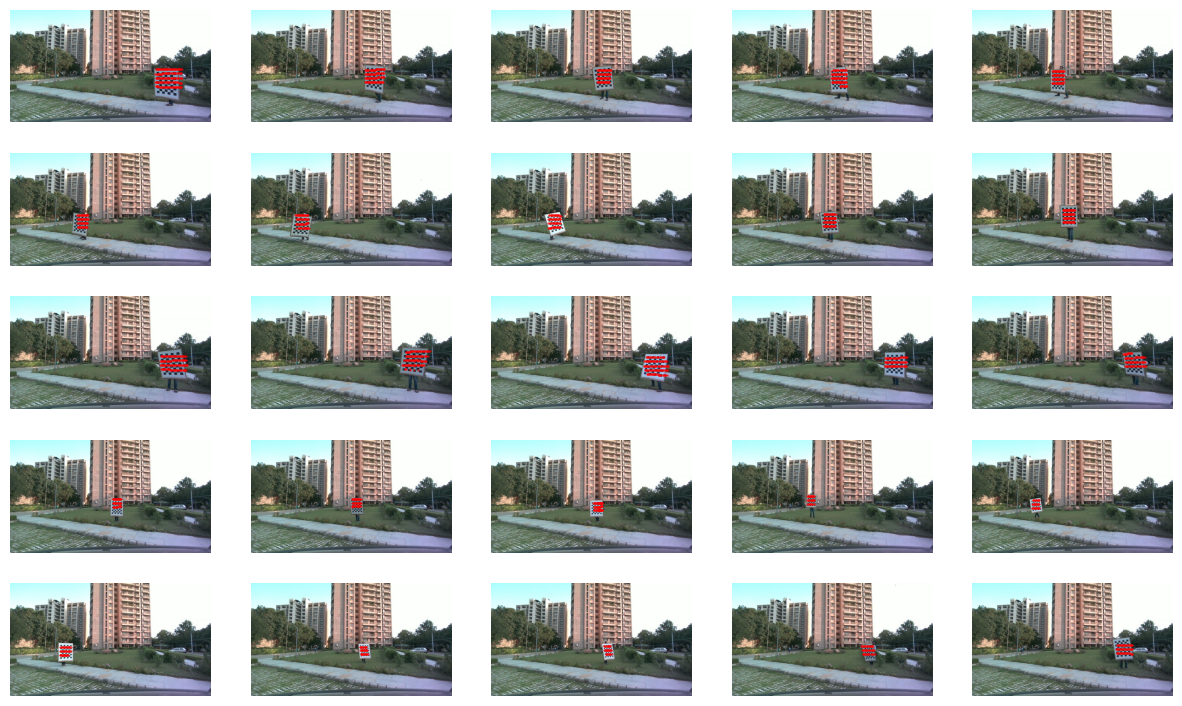
\includegraphics[width=0.875\textwidth]{Assets/Question-5/projection.png}
                \caption{LIDAR points projected to the image plane}
                \label{fig:lidar-projection}
            \end{center}
        \end{figure} \\
        It can be easily seen that not all points are within the checkerboard pattern's
        boundary. For example, in images 1 and 9, some of the projected points are to the
        right of the checkerboard. However, the points are close by. This could be due to
        the error in estimating the transformation matrix.

        \item We plot the normal vectors $\mathbf{\hat{n}}_{i}^{L}$, $\mathbf{\hat{n}}_{i}^{C}$,
        and $^{C} \mathbf{R}_{L} \mathbf{\hat{n}}_{i}^{L}$ for 5 selected images. The
        figure is given in \figref{normals-lidar}. In the figure, the blue normals are
        the LIDAR normals $\mathbf{\hat{n}}_{i}^{L}$, the green normals are the camera
        normals $\mathbf{\hat{n}}_{i}^{C}$, and the orange normals are the transformed
        LIDAR normals $^{C} \mathbf{R}_{L} \mathbf{\hat{n}}_{i}^{L}$.
        \begin{figure}[htbp]
            \begin{center}
                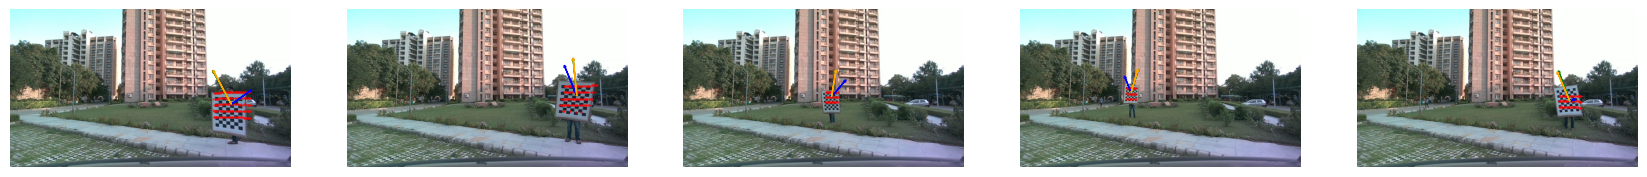
\includegraphics[width=0.875\textwidth]{Assets/Question-5/normals.png}
                \caption{Normal vectors for 5 selected images}
                \label{fig:normals-lidar}
            \end{center}
        \end{figure}
        \vspace*{0pt} \\
        It can be seen that the transformed LIDAR normals are close to the camera normals,
        whereas the plain LIDAR normals are not. This is expected, as the transformation
        matrix maps LIDAR points (and therefore vectors) to the camera coordinate frame.
        The normals were plotted on the chessboard pattern by finding the centroid of the
        LIDAR points, and then plotting an arrow from the centroid to a few units in the
        direction of the normal. \\
        We then calculate the cosine distance (normalized to $[0, 1]$) between the camera
        normals and the transformed LIDAR normals. Since the norm of the normals is 1, we
        simply take their dot product and scale it to $[0, 1]$. The distribution of these
        errors is given in \figref{cosine-distances}.
        \begin{figure}[htbp]
            \begin{center}
                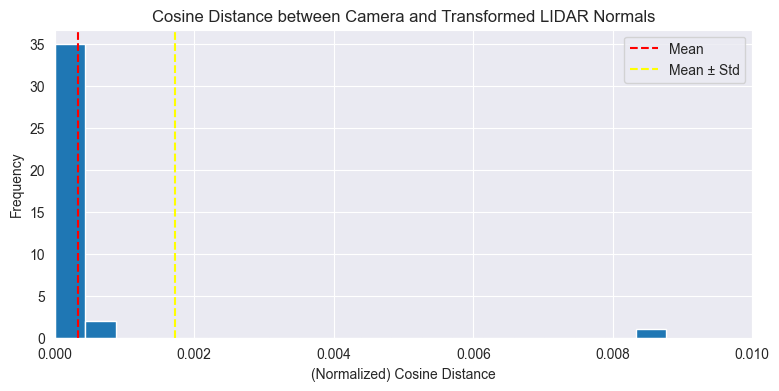
\includegraphics[width=0.875\textwidth]{Assets/Question-5/cosine-distances.png}
                \caption{Cosine distance between camera and transformed LIDAR normals}
                \label{fig:cosine-distances}
            \end{center}
        \end{figure}
        The mean cosine distance is $0.0003$, with a standard deviation of $0.0014$.
    \end{enumerate}

    \section*{\textbf{References}}
    \begin{enumerate}
        \item \href{https://learnopencv.com/camera-calibration-using-opencv/}{
            Camera Calibration using OpenCV
        }
        \item \href{https://www.ri.cmu.edu/pub_files/pub4/unnikrishnan_ranjith_2005_3/unnikrishnan_ranjith_2005_3.pdf}{
            Ranjith Unnikrishnan, Fast Extrinsic Calibration of a Laser Rangefinder to a Camera, 2005
        }
    \end{enumerate}

\end{document}